% Monografia de Projeto 1 e 2
% Alunos: David Candeia
%	  Diego Dantas
%	  Everton L. G. Alves
%         Felipe Coutinho
%
% Cliente: Hyggo Almeida
%
\documentclass[a4paper,titlepage,12pt]{report}

\usepackage{color}
\usepackage{longtable}
\usepackage[portuges,english]{babel}
%\usepackage[latin1]{inputenc}
\usepackage[utf8]{inputenc}
\usepackage{verbatim}
\usepackage{listings}
\usepackage{subfigure}

\usepackage{times}
%\usepackage[latin1]{inputenc}
\usepackage[utf8]{inputenc}
\usepackage[T1]{fontenc}
\usepackage{fancyhdr}
\usepackage{fancyvrb}

\usepackage{graphicx,url}
\usepackage{amssymb}
\usepackage{epsfig}


\sloppy
% Comandos de estilo e espacamento ----------------------------------------
\newlength{\defbaselineskip}
\setlength{\defbaselineskip}{\baselineskip}
\newcommand{\setlinespacing}[1]%
           {\setlength{\baselineskip}{#1 \defbaselineskip}}

\setcounter{topnumber}{2}
\renewcommand{\topfraction}{.7}
\setcounter{bottomnumber}{1}
\renewcommand{\bottomfraction}{.3}
\setcounter{totalnumber}{3}
\renewcommand{\textfraction}{.2}
\renewcommand{\floatpagefraction}{.5}
\setcounter{dbltopnumber}{2}
\renewcommand{\dbltopfraction}{.7}
\renewcommand{\dblfloatpagefraction}{.5}
%
\oddsidemargin -28pt
\evensidemargin -28pt
\marginparwidth 50pt
\marginparsep 5pt
\topmargin -27pt
\hoffset 15mm
\textheight 237mm
\textwidth 155mm
\renewcommand{\baselinestretch}{1.5}
%

%Listings ....
\lstset{numbers=left,
stepnumber=5,
firstnumber=1,
numberstyle=\tiny,
extendedchars=true,
breaklines=true,
frame=tb,
basicstyle=\footnotesize,
stringstyle=\ttfamily,
showstringspaces=false
}
\renewcommand{\lstlistingname}{Listagem}
\renewcommand{\lstlistlistingname}{Lista de Listagens}


% ------------------------------------------------------------------------

\begin{document}

% Primeira Folha do Documento %%%%%%%%%%%%%%%%%%%%%%%%%%%%%%%%%%%%%%%%%%%%%
\pagestyle{empty}

\begin{center}
{\textbf{\Large \textsc{Universidade Federal de Campina Grande}}}
\end{center}

\begin{center}
\textbf{{\Large \textsc{Centro de Engenharia Elétrica e
Informática}}}
\end{center}

\begin{center}
\textbf{{\Large \textsc{Unidade Acadêmica de Sistemas e
Computação}}}
\end{center}

\begin{center}
{\large \textsc{\textbf{Graduação em Ciência da Computação}}}
\end{center}


~\\


\begin{center}
{\Large \textsc{\textbf{Pyfinancial}}}
\end{center}
~\\

\begin{center}
\large{\textsc{David Candeia}\\ \textsc{Diego D. de Freitas}\\ \textsc{Everton L. G. Alves}\\
\textsc{Felipe L. Coutinho}}
\end{center}

% \begin{quote}
% \small{Monografia submetida à Coordenação do Curso de Ciência da
% Computação da Universidade Federal de Campina Grande - Campus I como
% resultado das disciplinas Projeto em Computação I e II.}
% \end{quote}
% ~\\
% 
% \begin{center}
% \textsc{Área de Concentração: Ciência da Computação }\\
% \textsc{Linha de Pesquisa: Processamento Digital de Imagens}\\
% \end{center}
~\\

\begin{center}
\textsc{Prof. Dr. Hyggo Almeida}\\
\textsc{(Orientador)}\\
\end{center}

~\\
~\\

\begin{center}
{\small \textsc{Campina Grande, Paraíba, Brasil}}\\
{\small \textsc{$\copyright$ David Candeia, Diego D. de Freitas, Everton L. G. Alves e Felipe L. Coutinho, 2009}}
\end{center}

%\newpage
\cleardoublepage



%%%%%%%%%%%%%%%%%%%%%%%%%%%%%%%%%%%%%%%%%%%%%%%%%%%%%%%%%%%%%%%%%%%%%%%%%%%%%%%%

\selectlanguage{portuges}

% Configura os n?meros das p?ginas para algarismos romanos
\pagestyle{plain}
\pagenumbering{roman}

% -------- Lista de Figuras --------- %

%\listoffigures
%\newpage

% ------------- ?ndice -------------- %
\tableofcontents
\newpage



\clearpage
%% Corpo do documento -------------------
%
% Configura os n?meros das p?ginas para algarismos indo-arabicos
\pagestyle{plain}
\setcounter{page}{1}
\pagenumbering{arabic}

\newenvironment{worduglystyle}[1]
{\spaceskip=.33em plus \hsize #1}
{}

%%%%%%%%%%%%%%%%%%%%%%%%%%%%%%%%%%%%%%%%%%%%%%%%%%%%%%%%%%%%%%%%%%%%%%%%%%%%%%%%%
%%% Definicao do cabecalho: secao do lado esquerdo e numero da pagina do lado direito
\pagestyle{fancy}
\addtolength{\headwidth}{\marginparsep}\addtolength{\headwidth}{\marginparwidth}\headwidth
= \textwidth
%\renewcommand{\sectionmark}[1]{\markboth{#1}{}}
\renewcommand{\sectionmark}[1]{\markright{\thesection\ #1}}\lhead[\fancyplain{}{\bfseries\thepage}]%
         {\fancyplain{}{\emph{\rightmark}}}\rhead[\fancyplain{}{\bfseries\leftmark}]%
             {\fancyplain{}{\bfseries\thepage}}\cfoot{}

%%%%%%%%%%%%%%%%%%%%%%%%%%%%%%%%%%%%%%%%%%%%%%%%%%%%%%%%%%%%%%%%%%%%%%%%%

\chapter{Introdução}

Exemplo de capítulo

\section{Teste 1}
\subsection{Teste 2}
\subsubsection{Teste 3}


\chapter{Fundamentação Teórica}

Matemática financeira é um ramo da Matemática que se utiliza de uma série de conceitos matemáticos para realizar a análise de dados financeiros em geral. Dentre deste ramo,  considerou-se na implementação da \textit{PyFinancial} os principais conceitos financeiros existentes na HP-12C \ref{glossario}.

É importante ressaltar que durante a pesquisa realizada no intuito de coletar as fórmulas financeiras relacionadas aos conceitos implementados, percebeu-se que várias são as fórmulas existentes e divulgadas na Internet, porém muitas delas não apresentam resultados similares aos da HP-12C. Com isso, à medida que são apresentados os conceitos será feita referência às fórmulas que estão implementadas e que se encontram no apêndice \ref{formulas}.

Abaixo tem-se uma breve explicação dos principais conceitos financeiros utilizados na \textit{PyFinancial}.

\section{Conceitos}

\subsection{Considerações iniciais}

Aplicações financeiras partem de um capital inicial e este é aplicado a uma certa taxa de juros, podendo ser esta aplicação ser configurada por uma série simples ou complexa, de modo a gerar, com o passar do tempo, um capital final que implique em alguma remuneração ou perda. Esses juros são aplicados ao capital de acordo com a capitalização fixada para o investimento. Como exemplos temos investimentos de poupança, empréstimos, etc.

Uma forma simples de ter-se uma idéia de como funciona uma dessas movimentações é observando o fluxo de caixa da mesma através de um diagrama de tempo. Um exemplo desse diagrama pode ser visto na figura \ref{tab:fig1}.

\subsection{Valor Presente - PV}

Aplicações têm início com uma quantia a partir de um marco inicial. Essa quantia corresponde a quanto vale o investimento inicialmente, sem análises do futuro. A esse valor, que pode ser um valor gasto ou recebido, damos o nome de valor presente ou valor atual. Um exemplo seria uma pessoa que aplica R\$ $500,00$ na poupança. Esse valor seria o valor presente de sua aplicação. Assim, valor presente, capital inicial e valor atual têm o mesmo significado.

O valor presente de uma dada prestação pode ser entendido como sendo o valor no instante zero de uma certa prestação futura descontada dos juros.

\subsection{Valor Presente Líquido - NPV}

Uma vez que o valor presente está definido, bem como as prestações, juros da movimentação e número de perídos durante o qual a aplicação estaŕa vigente, uma análise bastante comum é verificar qual o valor da aplicação atualmente. Ou seja, para cada prestação desconta-se o juros existente, seja este simples ou composto, considerando a quantidade de períodos até que a prestação fosse paga e obtém-se o valor da prestação na data-pólo inicial. Em seguida soma-se os valores presentes de cada prestação ao valor presente e obtem-se o NPV.

Um NPV positivo é um indicativo de que a aplicação possui um retorno positivo para o aplicante e que pode ser considerada. Já um NPV negativo indica que a aplicação não deve ser considerada.

Uma consideração importante a ser realizada é que esse valor presente líquido pode ser calculado de duas formas diferentes: uma com pagamentos postecipados e outra com pagamentos antecipados.

\subsection{Valor Futuro - FV}

Considerando o valor presente, os juros, as prestações e um dado período de vigência, o valor futuro de uma dada aplicação é o valor obtido ao final dessa aplicação. Ou seja, o valor futuro é o resultado da incidência dos juros e das prestações em cima do valor presente. Esse valor também é conhecido como capital final.

É importante destacar que, da mesma forma que o NPV, o valor futuro é influenciado pelo fato de estar-se trabalhando com pagamentos antecipados ou postecipados. Logo, dependendo do tipo de pagamento em vigência tem-se diferentes valores futuros.

\subsection{Taxa de juros - i e Taxa interna de retorno - irr}

Os juros, ou taxa de juros, de uma dada aplicação é o percentual que será aplicado sobre um montante de modo a gerar a remuneração da aplicação. Essa remuneração pode ser feita através de um sistema de juros compostos ou ainda de um sistema de juros simples.

A taxa interna de retorno, por sua vez, é a taxa de juros que iguala o valor presente das entradas ao longo da aplicação ao valor presente das saídas da aplicação. Ou seja, podemos entendê-la como o valor da taxa de juros que torno o valor presente líquido do investimento igual a zero, a aplicação não fez diferença.

Se a taxa de juros considerada para a aplicação for menor que o IRR então é um indicativo de que a aplicação é atrativa, se for maior a aplicação não deve ser considerada e sendo igual implica que a aplicação não fará diferença.

\subsection{Número de Períodos - n}

O número de períodos indica quantas vezes a taxa de juros será aplicada em uma certa aplicação de modo a gerar remuneração. Além disso, o número de períodos também informa os locais no tempo onde pode haver entradas ou saídas no fluxo, prestações.

\subsection{Prestações - pmt}

As prestações indicam entradas ou saídades de capital em um certo fluxo de caixa. Tipicamente nos cálculos considera-se uma prestação negativa para representar uma saída de capital e uma prestação positiva para representar uma entrada. Por exemplo, se pensarmos em uma empresa que recebe um montante de R\$ $60.000,00$ a cada ano e gasta um total de R\$ $20.000,00$, tem-se que o pmt a ser considerada para a aplicação da mesma é R\$ $40.000,00$.


\subsection{Sistema de amortização - SA}

Um sistema de amortização indica como um determinado financiamento é pago ao longo do tempo. Para isso define o valor das prestações que inclui tanto um montante a ser abatido do saldo devedor, bem como os juros a serem pagos. Assim, podemos entender como amortização a diminuição do saldo devedor, ou dívida, que pode ser realizada em etapas ou de uma única vez.

Dentre os sistemas de amortização mais famosos podemos citar o Sistema de Amortização Francês (SAF), ou Tabela Price, e o Sistema de Amortização Constante (SAC). Atualmente o SAC é bastante utilizado no Sistema de Financiamento Habitacional, em especial pela Caixa Econômica Federal, e o SAF é amplamente utilizado pelos bancos em seus sistemas de Crédito Direto ao Consumidor (CDC), bem como nas vendas a prazo divulgadas pelas grandes redes de varejo \cite{usoSACSAF}.



\chapter{Processo de Desenvolvimento}
asasa

\chapter{Análise de Requisitos}

\section{Modelo Conceitual}

% \begin{figure}[!h]
%  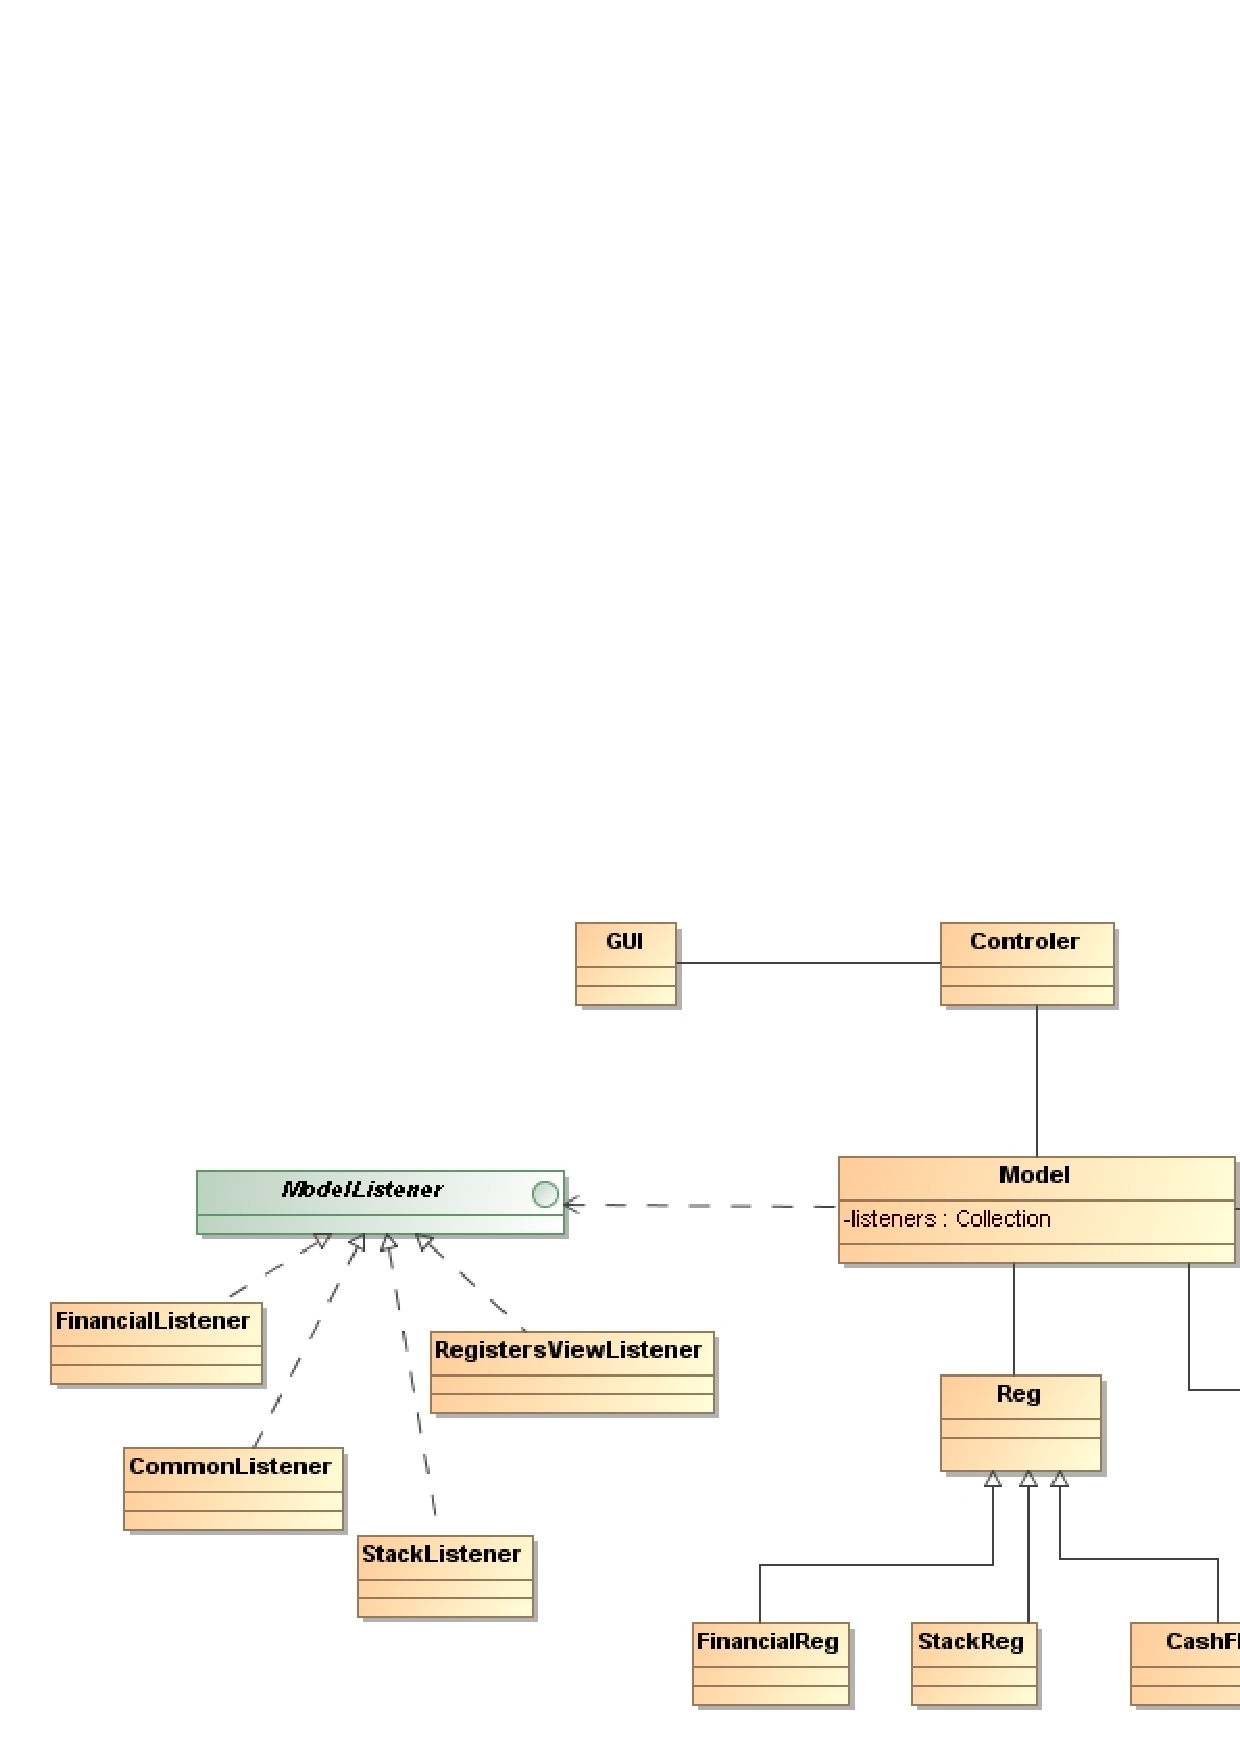
\includegraphics[height = 8cm]{CalcDC.jpg}
%  \caption{\it Modelo Conceitual da PyFinancial.} \label{fig:modConc}
% \end{figure}

\begin{figure}[!h]
 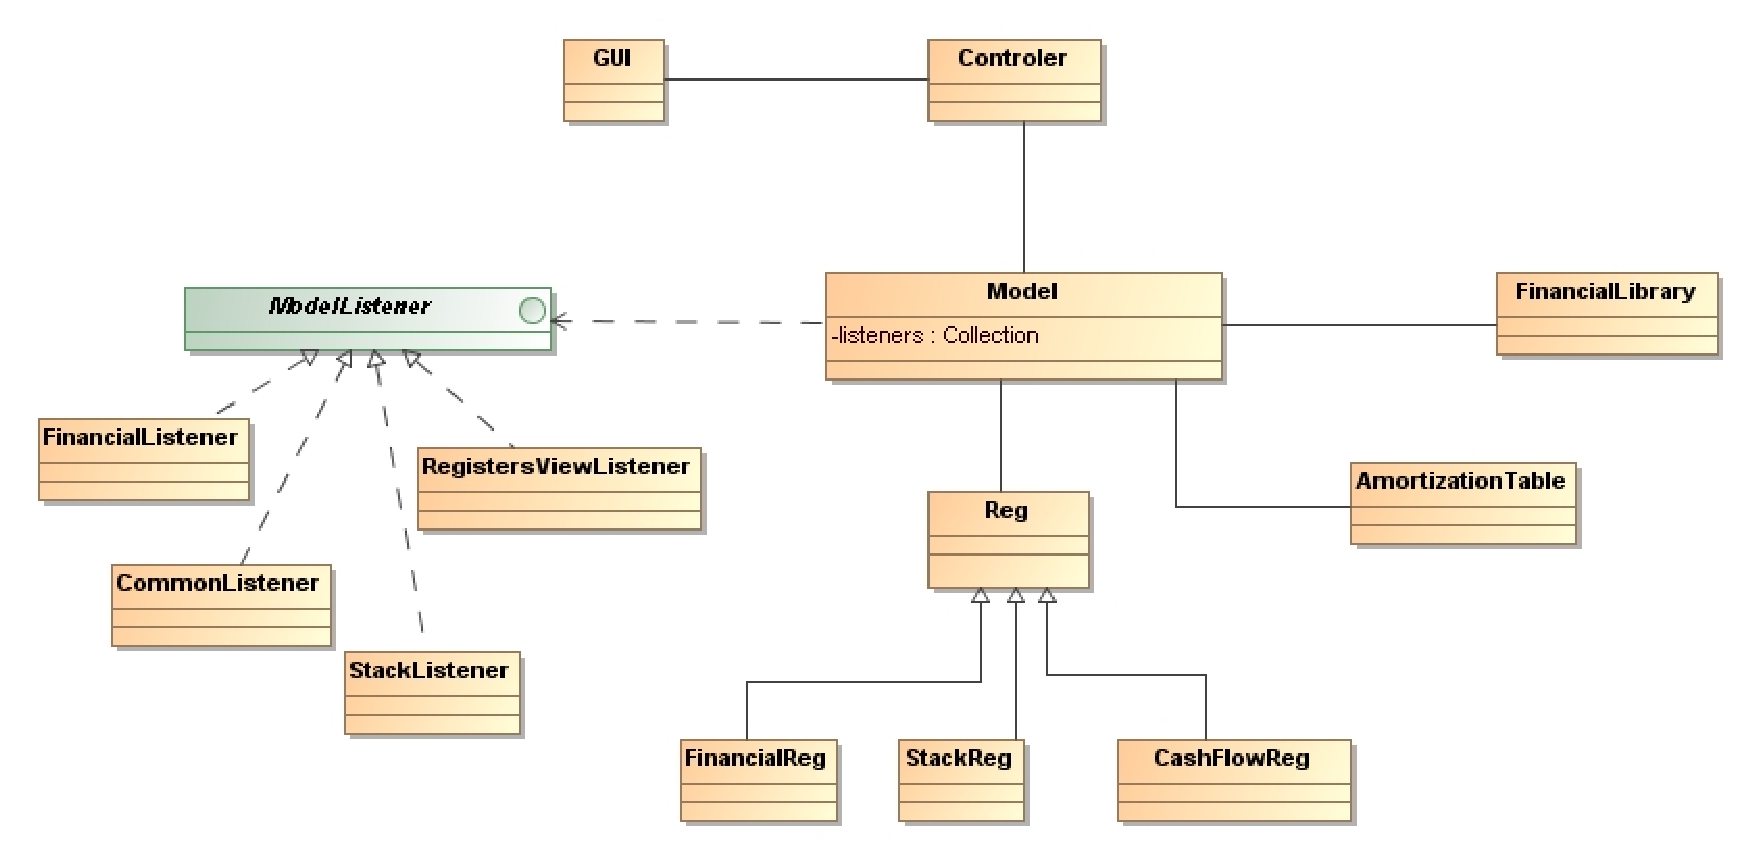
\includegraphics[scale=0.5]{CalcDC.eps}
 \caption{\it Tabela que descreve quando as atividades de XP1 devem ser realizadas.} \label{tab:modeConc}
\end{figure}

A figura \ref{tab:modeConc} apresenta o modelo conceitual da calculadora financeira, objetivo central desse projeto. É possível identificar algumas entidades centrais desse sistema são elas:

\begin{itemize}
	\item Model
	\item GUI
	\item Controler
	\item AbstractModelListener
	\item Reg
	\item FinancialLibrary
\end{itemize}

\subsection{Model}
Módulo central da aplicação que será responsável por fazer a troca de mensagens entre as demais entidades do sistema as quais está conectada, bem como realizar toda a manipulação de registradores (pilha, financeiros e demais registradores comuns) e funções de modo a efetivar as funcionalidades requisitadas pelo usuário. Também é de sua responsabilidade receber e preparar os dados da aplicação para posterior manipulação, dados esses captados pela interface. Por fim, esta entidade também é responsável por persistir os registradores quando necessário, bem como todo o estado interno da calculadora previamente configurada pelo usuário.

\subsection{GUI}
Esta é a entidade que estará em contato direto com o usuário da aplicação. Logo, este é o módulo que receberá os dados externos e os transmitirá para entidades mais internas, assim como receberá os resultados das operações realizadas pela calculadora e os transmitirá ao cliente de uma maneira mais amigável. Essa interface também é responsável por apresentar os dados segundo preferências do usuário previamente selecionadas, por exemplo, com um dado número de casas decimais.

\subsection{Controller}
Esta entidade é o controlador do sistema, responsável por desacoplar a interface da camada de negócios do sistema. Receberá as requisições feitas pelo cliente da aplicação, através da interface (\textit{GUI}), e identificará as operações correspondentes no \textit{Model} que se responsabilizarão por realizar as atividades correspondentes.

\subsection{AbstractModelListener}
Entidade abstrata da qual outras a generalizarão. Estas serão responsáveis por capturar qualquer mudança importante ocorrida no \textit{Model} que seja de interesse do usuário. Assim essas alterações serão refletidas na interface. Aqui encaixa-se situações como requisições de realização de operações matemáticas/financeiras, manipulações de registradores, etc.

\subsection{Reg}
Entidade que representa o papel de um registrador. Um registrador é um importante elemento usado para a realização das atividades objetivo da calculadora. Neles armazena-se os valores a serem utilizados nas operações, bem como os resultados das operações requisitadas. Esta entidade será especializada por outras adicionando as particularidades pertinentes aos diferentes tipos de registradores.

\subsection{FinancialLibrary}
Entidade que representa a biblioteca das funções financeiras. Todo e qualquer cálculo financeiro deve chamar a operação correspondente na biblioteca garantindo uma melhor organização e consequentemente, a separação de interesses.

Essa é a entidade que poderá vir a ser utilizada por programadores Python, incluindo os membros da equipe, para desenvolvimento das mais variadas aplicações que necessitem da realização de funções financeiras.

\section{Requisitos}

Durante as reuniões de planejamento entre os membros da equipe, o cliente e possíveis usuários dos nossos produtos, um conjunto de requisitos funcionais e não funcionais ficaram estabelecidos. São eles:

\begin{itemize}
 \item \textbf{Requisitos Funcionais}
	\begin{itemize}
 	\item O usuário deverá ser capaz de realizar as operações matemáticas/financeiras seguindo a Notação Polonesa Reversa \cite{NPR}.
	\item O usuário deve ser capaz de especificar o número de casas decimais apresentadas, bem como requisitar a apresentação dos valores em notação científica.
	\item O usuário deve ser capaz de adicionar/limpar valores em todos os 30 registradores existentes na calculadora. 
	\item O usuário deve ser capaz de realizar operações matemáticas básicas: soma ($+$),subtração ($-$), divisão ($/$) e multiplicação ($*$). Deve também ser capaz de realizar operações mais avançadas: exponenciação ($ e^{x} $), quadrado de um número ($x^{2}$), logaritmo natural ($\ln$), potência de números ($y^{x}$), raiz quadrada ($x^{1/2}$), percentual do total ($\%T$), variação percentual ($\Delta\%$) e percentual de um número ($\%$).
	\item O usuário deverá ser capaz de realizar cálculos que descubram os principais valores financeiros: número de períodos (n), taxa de juros (i), valor present (PV), valor da parcela (PMT) e valor futuro (FV). Esses cálculos podem envolver ou não multiplos fluxos de caixa.
	\item O usuário deve ser capaz de realizar análises de investimentos mais apuradas através do cálculo do valor presente líquido (NPV), bem como da taxa interna de retorno (IRR).
	\item O usuário deve ser capaz de calcular a amortização de suas dívidas no sistema de amortização francês (SAF), bem como no sistema de amortização constante (SAC). Apresentando uma tabela de amortização ao final.
	\item O usuário deve ser capaz de realizar a conversão entre taxas de juros anuais para taxas de juros mensais tanto no sistema de juros simples, como no sistema de juros compostos. Além disso, deve ser capaz de converter um número de períodos anuais em períodos mensais.
	\item O usuário deve ser capaz de rotacionar os valores dos registradores da pilha de cima para baixo.
	\item Ao finalizar o uso os dados da tela e dos registradores devem ser armazenados em algum tipo de persistência.
	
	\end{itemize}
 \item \textbf{Requisitos Não-Funcionais}
	\begin{itemize}
	 \item \textbf{Interface}. Possuir interface similar a da calculadora HP12-C, com melhoramentos que possam facilitar sua utilização.
	 \item \textbf{Usabilidade}. O nível de dificuldade encontrado para uso de nossa calculadora deve ser o mesmo encontrado quando faz-se uso das calculadoras tradicionais.
	 \item \textbf{Volume de Utilização}. A calculadora será mono-usuário, porém devendo ser robusta o suficiente para ser utilizada durante um longo intervalo de tempo ininterruptamente sem apresentar problemas.
	 \item \textbf{Hardware e software alvo}. A calculadora deverá funcionar no Internet Tablet N800 da Nokia, no sistema operacional Maemo Diablo (4.1.x) 
	 \item \textbf{Qualidade}. Com relação a precisão, deseja-se que os valores calculados em nossa calculadora não devam diferir em mais de $0.001$ unidades dos valores calculados na HP12-C original.
	 \item \textbf{Expressividade nas mensagens}. Entradas equivocadas do usuário deverão apresentar mensagens de erros que sejam mais intuitivas do que as apresentadas pela calculadora original (e.g. "Erro 6").
	 \item \textbf{Desempenho}. O tempo de resposta dos resultados não deve ultrapassar o tempo que a calculadora HP12-C leva para executar as mesmas operações (considerando que só o programa da calculadora esteja em execução).
	 \item \textbf{Segurança}. Os arquivos que conterão os valores dos registradores recém utilizados pelo usuário deverão ficar protegidos de alteração externa.
	 \item \textbf{Compatibilidade}. É desejável que a aplicação possa ser portada para versões mais novas do dispositivo alvo, como o N810, bem como para novas versões do Maemo.
	 \item \textbf{Internacionalização}. A calculadora deve ser desenvolvida para tornar possível a internacionalização. 
	 \item \textbf{Packaging}. A distribuição do aplicativo deve ser realizada através de um arquivo .deb que servirá como instalador para o mesmo.
	\end{itemize}
\end{itemize}


\chapter{Arquitetura}

% \begin{figure}[!h]
%  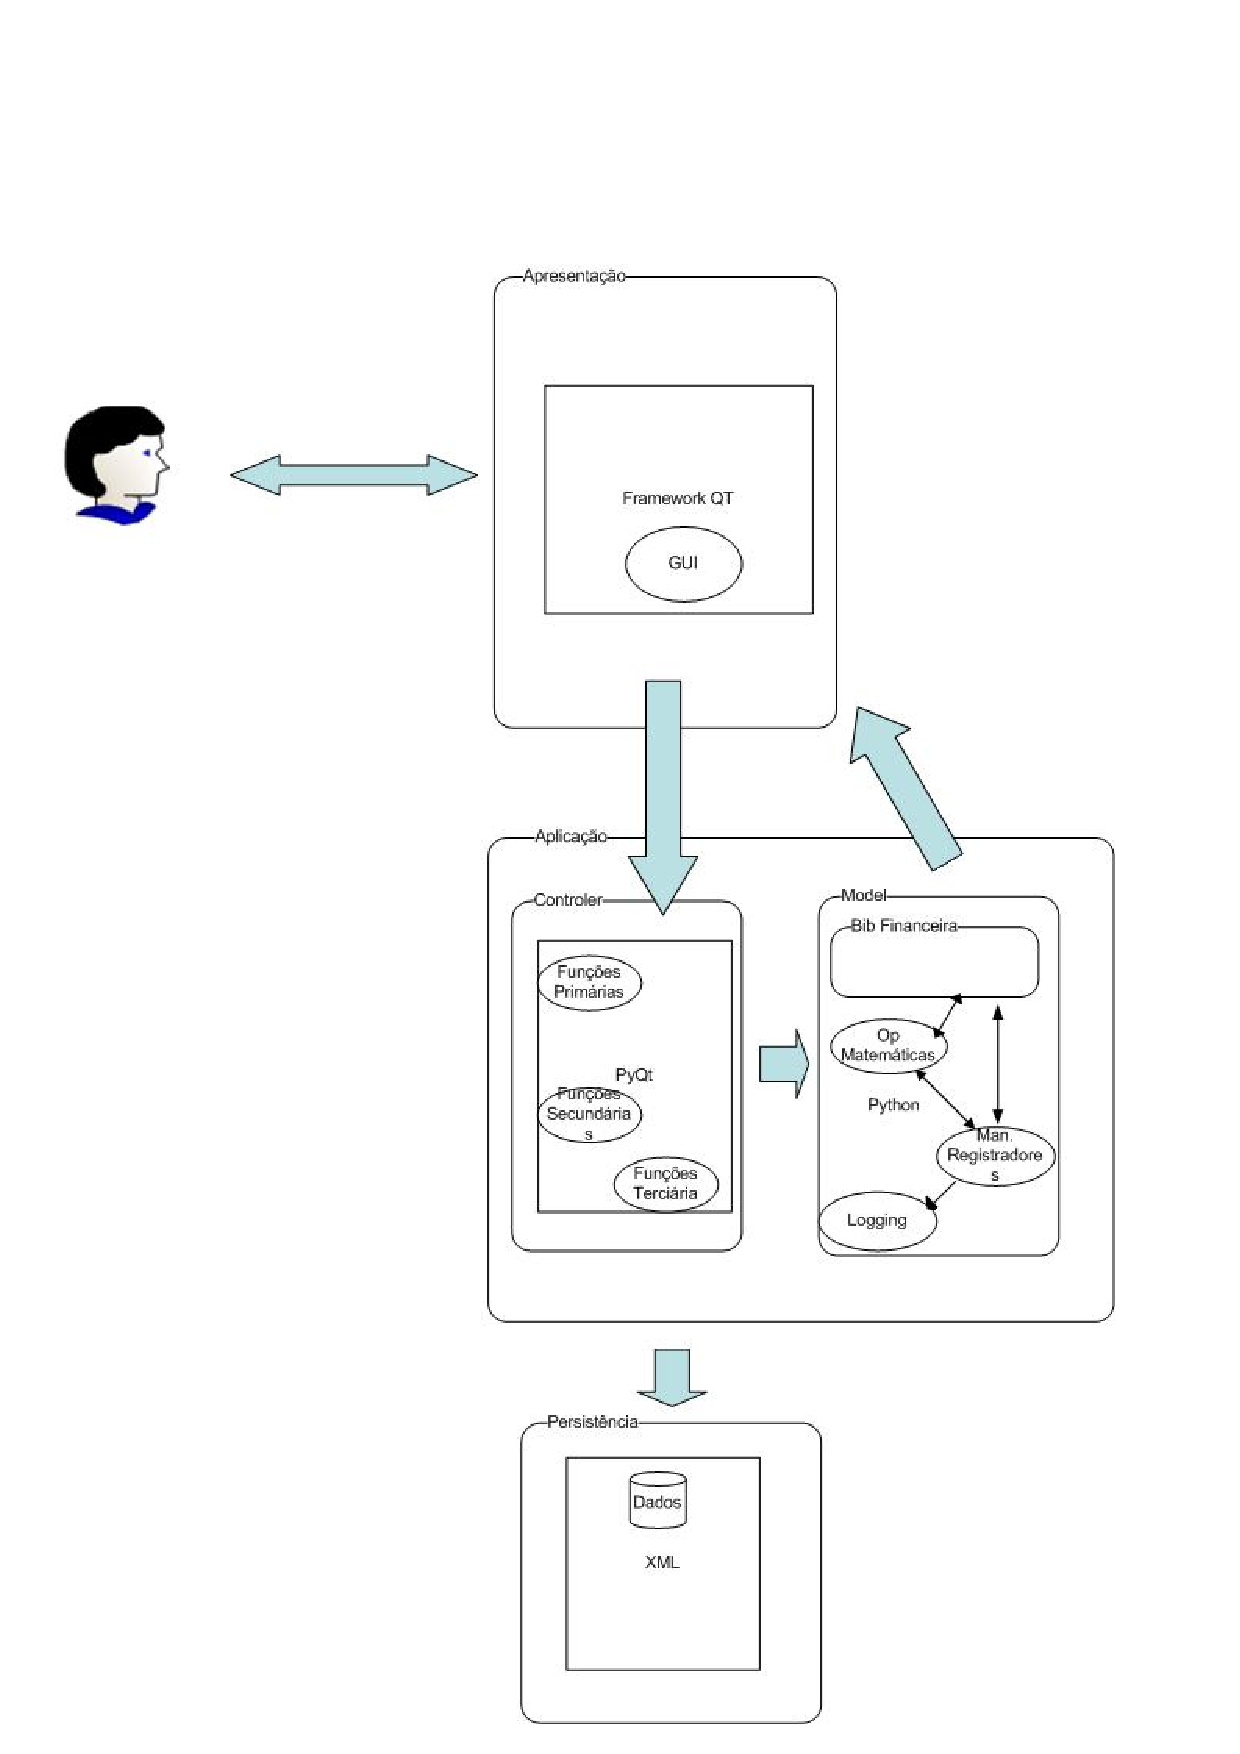
\includegraphics[scale=0.5]{arquitetura.jpg}
%  \caption{\it Projeto arquitetural da aplicação.} \label{fig:arquit}
% \end{figure}
\begin{figure}[!h]
 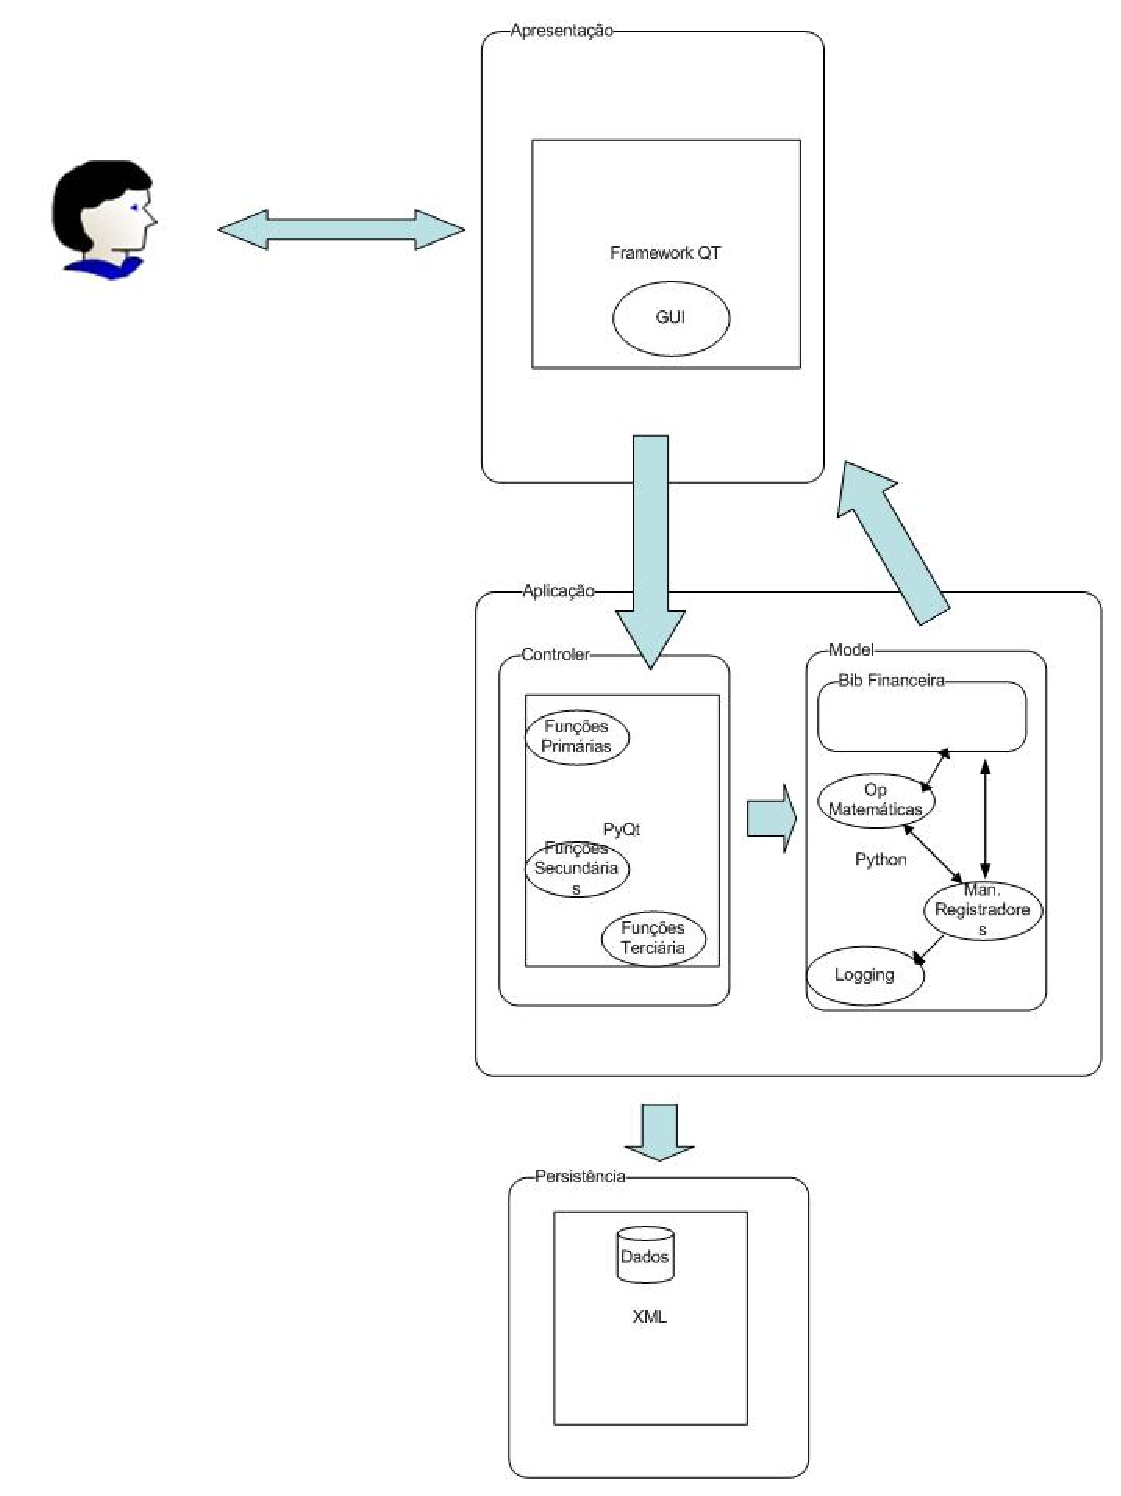
\includegraphics[scale=0.5]{arquitetura.eps}
 \caption{\it Projeto arquitetural da aplicação.} \label{fig:arquit}
\end{figure}

\section{Descrição da Arquitetura}
O sistema proposto foi idealizado para funcionar localmente no dispositivo N800 da Nokia, funcionando no modo monousuário. O sistema pode ser dividido, em três camadas lógicas que serão conectadas através do padrão MVC \cite{mvc}, conforme pode ser visto na Figura \ref{fig:arquit}:
\begin{itemize}
 \item \textbf{Apresentação}: camada que será responsável por lidar com todo aspecto de interface para interação com o usuário.
 \item \textbf{Aplicação}: camada que será responsável por conter toda a lógica do negócio de nossa aplicação, mantendo, assim total desacoplamento com as demais camadas.
 \item \textbf{Persistência}: camada que será responsável por lidar com toda a persistência de dados de mode que eles possam ser usados posteriormente íntegros.
\end{itemize}

Vale lembrar que toda a comunicação entre essas camadas, bem como entre os diversos módulos internos as mesmas, é realizada através de um conjunto de interfaces bem definidas, buscando assim, garantir flexibilidade e baixo acoplamento, bem como um eventual reuso e/ou substituição da biblioteca financeira em questão. A separação estre os módulos se deu da forma mais simplificada possível para que não existisse maior sobrecarga que pudesse influenciar drasticamente o tempo de resposta desejados para as iterações com o usuário da aplicação, este foi um dos requisitos não-funcionais especificados na fase de análise.
Outro ponto importante a se destacar é o uso do paradigma OO, bem como do uso de scripts, dada a escolha da linguagem Python para o desenvolvimento da Camada de Aplicação.

\subsection{Camada de Apresentação}
O sistema será acessado localmente por um único usuário via uma interface similar a da calculadora financeira que estamos usando como base, tendo a adição de menus de auxílio para uso do sistema e uma opção de finalização da aplicação. É importante destacar ainda que toda entrada realizada pelo usuário se dará através da interface touch-screen disponibilizada pelo dispositivo selecionado.
Para o desenvolvimento dessa camada faremos uso do Framework QT, com auxílio da ferramenta de design gráfico QT Designer. É de suma importância aqui o desenvolvimento de packages no que diz respeito aos componentes visuais da calculadora, por exemplo, os botões da mesma.

\subsection{Camada de Aplicação}
Como dito anteriormente, essa camada é responsável por toda a lógica de negócio de nosso sistema e foi desenvolvida em Python devido a suas vantagens na manipulação de números.
Dentre os principais componentes desta camada podemos dar destaque à biblioteca financeira (também desenvolvida por esta equipe com o foco de ser um módulo importável que contenha essencialmente funcionalidades financeiras), ao módulo de operações matemáticas, ao módulo de gerenciamento dos registradores existentes (responsável por fornecer os dados a serem persistidos) e ao módulo de comunicação com a interface da calculadora.
 Dentro dessa camada podemos destacar que as interações ocorrem em duas etapas:
\begin{enumerate}
 \item Numa primeira etapa teremos a comunicação dessa camada com a camada de apresentação do sistema através dos controladores, fazendo estes uso dos bindings em PyQt e sendo subdivididos de acordo com as funcionalidade providas por cada tecla.
 \item Numa segunda etapa teremos:	
 \begin{itemize}
  \item \begin{itemize}
         \item A comunicação dos módulos controladores com o restante da lógica da aplicação, fazendo uso das funcionalidades da biblioteca financeira, do módulo matemático e manipulando os seus registradores.
	 \item A interação entre os registradores e a biblioteca, onde os primeiros podem fornecer entradas para a última, a interação entre os registradores e o módulo matemático e a interação entre o módulo matemático e a biblioteca.
        \end{itemize}
 \end{itemize}
\end{enumerate}

\subsection{Camada de Persistência}
A persistência dos dados relativos aos registradores é realizada através do uso de arquivos. Os dados que forem armazenados nos arquivos deverão ser recarregados sempre que houver a inicialização da aplicação, demandando, assim, pouca interação com o disco.
Outro aspecto relevante a ser considerada aqui é a segurança do sistema.  Devido à natureza do sistema focamos nos aspectos de integridade dos dados manipulados, fazendo com que os arquivos utilizados fossem armazenados de forma oculta ao usuário, evitando, assim, alterações dos mesmos por parte deste.

\subsection{\textit{Packing}}
Foi tomada a decisão de distribuir a aplicação através de um arquivo de instalação de extensão .deb, simplificanco assim a maneira de intalação do software. Tal arquivo poderá ser obtido por download de certo servidor web que será escolhido pela equipe em conjunto com o cliente.

\subsection{Pontos Adicionais}
Com relação à integração com outras aplicações, é do interesse da equipe que a biblioteca financeira desenvolvida possa vir a ser usada por outros desenvolvedores como um dos vários módulos que auxiliem sua aplicação específica.
Por fim, todo nosso desenvolvimento foi guiado pelo padrão de operações que é usado pela HP12-C que é a Notação Polonesa Reversa, ou Inversa segundo alguns autores \cite{NPR}



\chapter{Verificação e Validação}
dsdsd


\input{./files/metricas}

\chapter{Conclusões}

\section{teste}

asassd ....


\appendix
\chapter{Glossário} \label{glossario}

\textbf{A}

\begin{itemize}
\item Amortização:
    A palavra amortização pode ser entendida como a diminuição da dívida, de uma única vez ou aos poucos, em mais vezes. 
\end{itemize}

\textbf{C}
\begin{itemize}
\item Capitalização: 
    Periodicidade do vencimento do juro ou número de vezes em que o juro é processado (calculado) num ano: anual, semestral, trimestral, mensal, etc. 

\item Capitalização Linear:
    A capitalização linear – ou método de formação dos juros simples – considera a incidência periódica de uma dada taxa de juros sobre uma base de cálculo fixa. 

\item Capitalização exponencial:
    A capitalização exponencial ou – método de formação dos juros compostos – considera a incidência periódica de uma dada taxa de juros sobre uma base de cálculo variável. 

\item Capital inicial:
    Capital existente na data-pólo inicial. 

\item Capital final:
    Capital existente na data-pólo final. 

\end{itemize}

\textbf{D}
\begin{itemize}
 \item Data-pólo inicial:
    Data de início do investimento. 

\item Data-pólo final:
    Data de resgate do investimento. 

\item Datas-focais intermediárias:
    Datas localizadas entre a data-pólo inicial e a data-pólo final, onde existem movimentações financeiras. 

\item Diagrama de tempo:
    Diagrama que apresenta o fluxo de caixa juntamente com os instantes de tempo das movimentações. Por convenção, recebimentos, entradas ou fluxos positivos são representados por setas apontando para cima ao passo que saídas ou pagamentos ou fluxos negativos são representados por setas apontando para baixo. 
\end{itemize}

\textbf{F}
\begin{itemize}
 \item Fluxo de Caixa:
    Montante de caixa recebido e gasto por uma entidade durante um período de tempo definido, algumas vezes ligado a um projeto específico. 
\end{itemize}

\textbf{J}
\begin{itemize}
 \item Juros de uma prestação em um sistema de amortização:
    Quantia paga além do valor amortizado em cada parcela. É calculada em função da taxa de juros e do saldo devedor do instante anterior. 

\item Juros Simples:
    No sistema de juros simples, os juros são calculados sobre o principal da dívida (valor inicial emprestado ou aplicado).

\item Juros Compostos:
    No sistema de juros compostos, os juros de cada período somam-se à dívida, incidindo juros sobre ele no período seguinte.
\end{itemize}

\textbf{P}
\begin{itemize}
 \item Pagamento Antecipado:
Pagamento de uma prestação que é realizado no início de um dado período.

\item Pagamento Postecipado:
Pagamento de uma prestação que é realizado no término de um dado período.

\item Prestação:
    Instrumento de recuperação ou de devolução de um capital acrescido dos juros contratados no período de negociação da transação. 
\end{itemize}

\textbf{S}
\begin{itemize}
 \item Saldo Devedor:
    Montante que ainda necessita ser abatido em um dado instante de tempo considerando um certo sistema de amortização. 

\item Série Simples:
    Quando um fluxo de caixa apresenta apenas datas-pólo, ou seja, temos apenas dois fluxos. 

\item Série Complexa:
    Quando um fluxo apresenta ao menos uma data-focal intermediária além das datas-pólo, ou seja, tem-se no mínimo três fluxos. 

\item Série Uniforme de Prestações Uniformes:
    Conjunto de pagamentos ou recebimentos nominais iguais, dispostos em períodos constantes ao longo de uma série complexa de fluxo de caixa. Pode ser de três tipos: postecipada, antecipada ou diferida. 

\item Série Uniforme de Prestações Uniformes Antecipada:
    São pagamentos ou recebimentos distribuídos por todos os períodos de uma série complexa de fluxo de caixa, inclusive na data-pólo inicial ou data-focal zero. 

\item Série Uniforme de Prestações Uniformes Diferida:
    São pagamentos ou recebimentos distribuídos em uma série complexa de fluxo de caixa por períodos situados após um determinado prazo de carência. 

\item Série Uniforme de Prestações Uniformes Postecipada:
    São pagamentos ou recebimentos distribuídos por todos os períodos de uma série complexa de fluxo de caixa, menos na data-pólo inicial ou data-focal zero. 

\item Sistema de Amortização:
    É a forma pela qual são calculadas as prestações que você vai pagar no decorrer do financiamento. Nos empréstimos de longo prazo, esses pagamentos são, normalmente, efetuados por parcelas (prestações), compostas de cotas de amortização e de juros. 

\item Sistema de Amortização Constante:
    É um método onde as amortizações do capital apresentam comportamento uniforme ou constante durante o período de vigência de uma operação financeira. Os juros apresentam valores heterogêneos e decrescentes ao longo do tempo, o que resulta em prestações heterogêneas e decrescentes ao longo do tempo. 

\item Sistema de Amortização Mista:
    Criado em 1979 pelo BNH. Representa um plano de amortização misto, a partir da combinação entre os sistemas Francês e Constante, onde juros, amortização e prestação, derivam de médias aritméticas envolvendo os valores calculados no PRICE e no SAC. Os juros apresentam valores heterogêneos e decrescentes ao longo do tempo. Com os juros heterogêneos e amortizações homogêneas temos uma configuração de prestações heterogêneas e decrescentes. 

\item Sistema Francês:
    Criado no século XVIII pelo matemático, filósofo e teólogo inglês Richard Price (por isso o nome Sistema Price), é um método de amortização com prestações iguais e vencidas, onde juros e amortizações portam-se de maneiras decrescente e crescente. 
\end{itemize}

\textbf{T}
\begin{itemize}
\item Taxa de Juros:
    É o percentual que remunera o capital. Uma taxa de juros incide sobre um capital disposto em um fluxo de caixa sempre quando da ocorrência de uma variação temporal, conhecida como freqüência intervalar necessária à formação dos juros. 
\end{itemize}

\textbf{V}
\begin{itemize}
 \item Valor Atual ou Valor Presente:
    Representa um fluxo qualquer situado na data-pólo inicial. 

\item Valor Nominal
    Representa um fluxo qualquer situado entre a data-focal intermediária 1 e a data-pólo final. 

\item Valor Futuro Antecipado:
    Representa o somatório de todas as prestações capitalizadas à data-pólo final, com uma mesma taxa de juros; o PMT contido na data-pólo final não sofre nenhuma alteração 

\item Valor Futuro Postecipado:
    Representa o somatório de todas as prestações capitalizadas à data-pólo final, 
com uma mesma taxa de juros.

\item Valor Presente Antecipado:
    Representa o somatório de todas as prestações descontadas à data-pólo inicial, com uma mesma taxa de juros; o PMT data-pólo inicial não sofre nenhuma alteração. 

\item Valor Presente Postecipado:
    Representa o somatório de todas as prestações descontadas à data-pólo inicial, com uma mesma taxa de juros. 
\end{itemize}
\chapter{Fórmulas}

Aqui serão apresentadas as fórmulas usadas, bem as fontes a partir das quais as mesmas foram obtidas: \\

\begin{enumerate}
 \item pv - BEG \cite{arachnoid}:

\begin{eqnarray*}
pv &=& (i+1)^{-n} * ( -fv*i - (i+1) * ( (i+1)^{n} -1)*pmt  ) / i\\
\end{eqnarray*}

% Fonte: http://www.arachnoid.com/lutusp/finance.html

\item pv - END \cite{arachnoid}:

\begin{eqnarray*}
	pv &=& (i+1)^{-n} * ( -pmt*(i+1)^{n} - fv*i + pmt) / i \\
\end{eqnarray*}

%  Fonte: http://www.arachnoid.com/lutusp/finance.html

\item pv com i = 0 \cite{matFinanceira}: 

\begin{eqnarray*}
  pv &=& fv + n * pmt  \\
\end{eqnarray*} 

% Fonte: Material de Camilo e \cite{matFinanceira}

\item fv - BEG \cite{arachnoid}:
\begin{eqnarray*}
 fv &=& ( (i+1)*pmt - (i+1)^{n}*(i*pmt + pmt + i*pv) ) / i \\
\end{eqnarray*}

%  Fonte: http://www.arachnoid.com/lutusp/finance.html

\item fv - END \cite{arachnoid}: 
\begin{eqnarray*}
fv &=& ( pmt - (i+1)^{n} * (pmt + i*pv) ) / i \\
\end{eqnarray*}

%  Fonte: http://www.arachnoid.com/lutusp/finance.html 

\item fv com i = 0 \cite{arachnoid2}:
\begin{eqnarray*}
 fv &=& - (pv + n*pmt) \\
\end{eqnarray*}
 
%  Fonte: Material de Camilo e \cite{matFinanceira}

\item  n - BEG \cite{arachnoid}:
\begin{eqnarray*}
 n &=& log( (-fv*i + pmt*i + pmt) / (i*pmt + pmt + i*pv) ) / log(i+1) \\
\end{eqnarray*} 

%   Fonte: http://www.arachnoid.com/lutusp/finance.html 

\item  n - END \cite{arachnoid}: 
\begin{eqnarray*}
 n &=& log( (pmt - fv*i) / (pmt + i*pv) ) / log(i+1) \\
\end{eqnarray*} 
  
%  Fonte: http://www.arachnoid.com/lutusp/finance.html

\item  n com i = 0 \cite{arachnoid2}: 

\begin{itemize}
 \item Se pólos com sinal igual:
	\begin{eqnarray*}
 		 n &=& |(pv - fv)| / |pmt| \\ 		
	\end{eqnarray*}
  \item c.c:
	\begin{eqnarray*}
 		n &=& (|pv| - |fv|) / |pmt|   ^{1} \\	 
	\end{eqnarray*}
\end{itemize}
 
%  Fonte: Material de Camilo e \cite{matFinanceira} \\

\item  pmt - BEG \cite{arachnoid}: 
\begin{eqnarray*}
	pmt &=& - i*( pv* ( i+1 )^{n} + fv ) / ( (i+1)*( (i+1)^{n} - 1 ) ) \\
\end{eqnarray*} 
 
%  Fonte: http://www.arachnoid.com/lutusp/finance.html \\ 

\item  pmt - END \cite{arachnoid}:
\begin{eqnarray*}
	pmt &=& - i*( pv*(i+1)^{n} + fv ) / ((i+1)^{n} - 1) \\	
\end{eqnarray*}  
 
%  Fonte: http://www.arachnoid.com/lutusp/finance.html \\

\item  pmt com i = 0 \cite{arachnoid2}:  

\begin{itemize}
 \item Se pólos com sinal igual:
	\begin{eqnarray*}
 		 pmt &=& |(pv - fv)| / |n| \\	
	\end{eqnarray*}
  \item c.c:
	\begin{eqnarray*}
 		pmt &=& (|pv| - |fv|) / |n|  ^{1} \\	 
	\end{eqnarray*}
\end{itemize}

%  Fonte: Material de Camilo e \cite{matFinanceira}  

\item  i: Usa-se a função do fv com estimativas de i $ ^{2} $  \cite{arachnoid2}

%  Fonte: http://vps.arachnoid.com/finance/

\item  npv \cite{man1}:
\begin{eqnarray*}
 	NPV &=& CF_{0} + CF_{1} / (1+i)^{1} + CF_{2} / (1+i)^{2} + ... + CF_{n} / (1+i)^{n} \\
\end{eqnarray*}
 
%  Fonte: Manual da HP c00363319

\item  irr \cite {matFinanceira2}: Resolvido por iteração da fórmula acima até que $ NPV = 0. $ 

%  Fonte: Matemática Financeira de Samuel Hazzan e José Nicolau Pompeo

\item SAF: pmt \cite{adail}
\begin{eqnarray*}
 	pmt &=& pv * (1+i)^{n} * i / ((1+i)^{n}-1) \\
\end{eqnarray*}
 
%  Fonte: Material Adail

\item  SAF: amort \cite{adail}
\begin{eqnarray*}
 	A_{t} &=& (pmt - (pv*i)) * (i+1)^{t-1} \\	
\end{eqnarray*}
 
%  Fonte: Material Adail

\item  SAC: juros \cite{adail}
\begin{eqnarray*}
 	J_{t} &=& pv*i - (A_{t}*i*t-1)	
\end{eqnarray*}
 
%  Fonte: Material Adail 

\item  SAC: pmt \cite{adail}
\begin{eqnarray*}
 	pmt_{t} &=& A_{t} + J_{t}	\\
\end{eqnarray*}
 
%  Fonte: Material Adail

\item  SAC: amort \cite{adail}

\begin{eqnarray*}
 	A_{t} &=& pv / n \\	
\end{eqnarray*}
 
%  Fonte: Material Adail

\item  Conversão do n \cite{man2}:
\begin{eqnarray*}
 	n_{mensal} &=& n_{anual} * 12 \\	
\end{eqnarray*}
 
%  Fonte: Manual da HP Platinum em Português

\item  Conversão do i (juros simples) \cite{camilo}:
\begin{eqnarray*}
 	i_{mensal} &=& i_{anual} / 12 \\	
\end{eqnarray*}
  
%  Fonte: Material de Camilo de taxas equivalentes

\item  Conversão do i (juros compostos) \cite{camilo}:
\begin{eqnarray*}
 	i_{mensal} &=& (1+i_{anual})^{1/12} - 1 \\	
\end{eqnarray*}
 
%  Fonte: Material de Camilo de taxas equivalentes

\item Percentagem de um dado valor \cite{man1}:
\begin{eqnarray*}
 	\% &=& Base(y) * Rate(x) / 100 \\	
\end{eqnarray*}

\item Variação Percentual \cite{man1}:
\begin{eqnarray*}
 	\Delta\% &=& 100*(NewAmount(x)-Base(y))/Base(y) \\	
\end{eqnarray*}

\item Percentagem do Total \cite{man1}:
\begin{eqnarray*}
 	\%T &=& 100*(Amount(x)/Total(y)) \\	
\end{eqnarray*}

\end{enumerate}

Observações: 

$ ^{1} $ : Faz-se ainda um novo cálculo do pv com o valor resultante do n. Se o valor retornado for diferente, inverte-se o sinal do n.

$ ^{2} $ : O algoritmo base inicia com uma taxa de juros de 100\% e iterativamente, no máximo duas iterações mais externas trocando o sinal da taxa ou até achar a solução busca-se um novo valor de i. Internamente tenta-se acrescer uma estimativa atual de um valor gd, alterado de 0.5 ou -0.5 de acordo com certas condições, e verifica-se a proximidade do resultado dessa estimativa na função do fv em relação ao valor real do fv. Realizando-se três tentativas consecutivas de cálculo de fv que fiquem com um erro inferior a $ 1e-8 $ para-se o algoritmo, ou então tenta-se um número máximo de 400 iterações internas em estimativas do i.
\chapter{Novas Funcionalidades}

Um das características de um software bem projetado é permitir facilmente a inclusão de novas funcionalidades. 
Aqui será apresentado os passos necessários para a inclusão de novas funcionalidades.

Antes de apresentar o passo-a-passo, deve-se levantar as seguintes considerações:

\begin{enumerate}
 \item Em relação a interface gráfica, o módulo principal que organiza os dados de interface gráfica da calculadora, 
incluindo disposição de botões, é o CalcGui. Além desse, existem módulos que lidam com a tabela de amortização 
(calcTabelDialog), com a tabela de recall (recallViewDialog), com a tabela de store (storeViewDialog) e a 
representação genérica de um botão (calcButton).

\item Existe um componente que representa um botão (calcButton), podendo esses ter adicionados até 3 textos de 
funções: uma na parte superior, um na parte inferior e um na parte central.

\item O controller (calcController) captura todos os eventos de teclas pressionadas, considerando o texto da parte central do botão 
(que representa a função principal de cada tecla). Em seguida chama uma ação correspondente no model (calcModel)

\item O calcModel é a facade do model do sistema e guarda o estado da calculadora (opções de arredondamento, 
se as teclas especiais f ou g estão pressionadas, etc) e conhece a pilha (calcStack), os demais registradores (calcRegs) 
e as funções da biblioteca financeira (pyFinancialLibrary).

\item As várias funções presentes em calcModel representam chamadas as teclas de uma dada função principal 
(a funcão cujo texto fica no meio do botão). Dado que o model conhece o estado da calculadora, em cada uma dessas 
chamadas verifica-se que função da biblioteca usar verificando o estado de F e G.

\item Na ligação do modelo, da interfaçe gráfica e do controlador foi utilizado o modelo MVC \cite {mvc}. 
Os módulos da interface gráfica funcionam como observers. O model tem vários listeners para eventos como: 
modificação do valor da tela, modificação da pilha, etc. Ao final de cada função do model, faz-se as ações necessárias 
(desativar F ou G pressionados; avisar listeners sobre alterações na pilha, registradores financeiros, etc, 
dependendo do que a função faça; alertar a interface sobre modificação na tela, no estado dos botões ou sobre 
a necessidade de mostrar a tabela de amortização, de recall ou de store.

\item Os dados fornecidos de volta aos listeners estão sempre no formato de Decimal, que é o tipo trabalhado pela 
calculadora de modo a alcançar alta precisão. Cada módulo da GUI formata esses dados como queira, usando os métodos 
de formatacão do módulo calcFormatUtil.

\end{enumerate}

Agora, como exemplo, irá se utilizar a implementação de uma nova forma de divisão em que ao invés de se dividir o 
registrador Y pelo X, irá se dividir X por Y. Através desse exemplo, pretende-se abordar todo o passo-a-passo para se 
implementar uma nova funcionalidade.

Primeiramente é preciso escolher um botão do teclado da GUI que esteja livre para receber a nova função. 
No método \begin{verbatim} __createKeyboardLayout \end{verbatim}
do módulo calcGui é feita a adição do botões na tela. Escolha uma posição e adicione o 
botão através de \begin{verbatim}self.__addGridButton(grid, "INV /", 1, 5)\end{verbatim}

Agora, criar a ação relativa ao botão no método \textbf{keyboardButtonClicked(self, text)}
do controller: 

\lstinputlisting[language=Python, label=else, caption={Teste no controller}]{else.py}
% \begin{verbatim}
% 	elif text == "INV /":
%  		self.__model.invDiv()
% \end{verbatim}

No model, criar o método chamado no controller. Nele, implementar a nova funcionalidade baseado nos valores de 
F e G, nos valores dos registradores e no estado da calculadora. Com o resultado da divisão em mãos, setar algum dos 
registradores conforme necessário. Desativar as teclas F e G, e conforme o que for modificado (tela, pilha, registradores 
financeiros, etc) avisar os devidos listeners sobre as alterações. Um ponto importante é também alterar o modo de 
entrada de dados da calculadora de acordo com a funcionalidade desejada. Existem basicamente três modos: 
Mode.SaveMode (que devolve o valor 0.0 a tela), Mode.OperationMode (devolve zero a tela, mas antes dá um enter na pilha) 
e Mode.EntryMode (que indica que números estão sendo entrados na tela).

\lstinputlisting[language=Python, label=funcao, caption={Definição de Função no Model}]{funcao.py}


% \begin{verbatim}
% 
%     def invDiv(self):
%         if self.__isGPushed or self.__isFPushed:
%             self.__fireException("Function not yet implemented.")
%             self.__deactiveFandG()
%         else:
%             # "inv /"
%             try:
%                 result = self.__calcStack.getXReg() / self.__calcStack.getYReg()
%                 self.__calcStack.rollCounterClockWise()
%                 self.__calcStack[0] = result
%                 self.__calcStack[3] = self.__calcStack[2]
%         
%                 self.mode = Mode.OperationMode
%                 self.base = None
%                 self.dotActived = False
%         
%                 self.__fireStackRegisters(self.getAllStackRegisters())
%                 self.__fireScreenChangedEvent()
%                  
%             except Exception, e:
%                 self.__fireException(e.message)
% \end{verbatim}

\chapter{Tabela de Erros} \label{tabelaErros}

Como sabe-se sistemas apresentam restrições quanto as entradas fornecidas de modo a realizar determinadas atividades. Na HP-12C entradas inválidas produzem erros que são apresentados ao usuário através de um código no formato \textbf{ERROR d+}, onde d+ indica um ou mais dígitos. Esse formato dificulta o entendimento por parte do usuário do motivo que levou ao erro, ou seja, o usuário necessita ter em mãos o manual da calculadora que explicita o significado do código visualizado.

Nesse sentido, buscou-se fazer uso das facilidades que o dispositivo computacional em foco oferece de modo a melhorar a usabilidade do sistema. Para isso foi realizado um mapeamento dos códigos de erros encontrados nos cálculos financeiros na HP-12C para mensagens de texto que explicitem melhor o problema encontrado. 

Como a aplicação desenvolvida é composta de uma biblioteca financeira que é utilizada pela aplicação calculadora financeira, optou-se por realizar dois mapeamentos: um das mensagens que são geradas pelos cálculos financeiros da biblioteca e outro das mensagens que são geradas por estados inconsistentes na calculadora. Tais mapeamentos estão presentes nas tabelas \ref{tabErros1} e \ref{tabErros2}.

\begin{figure}[!h]
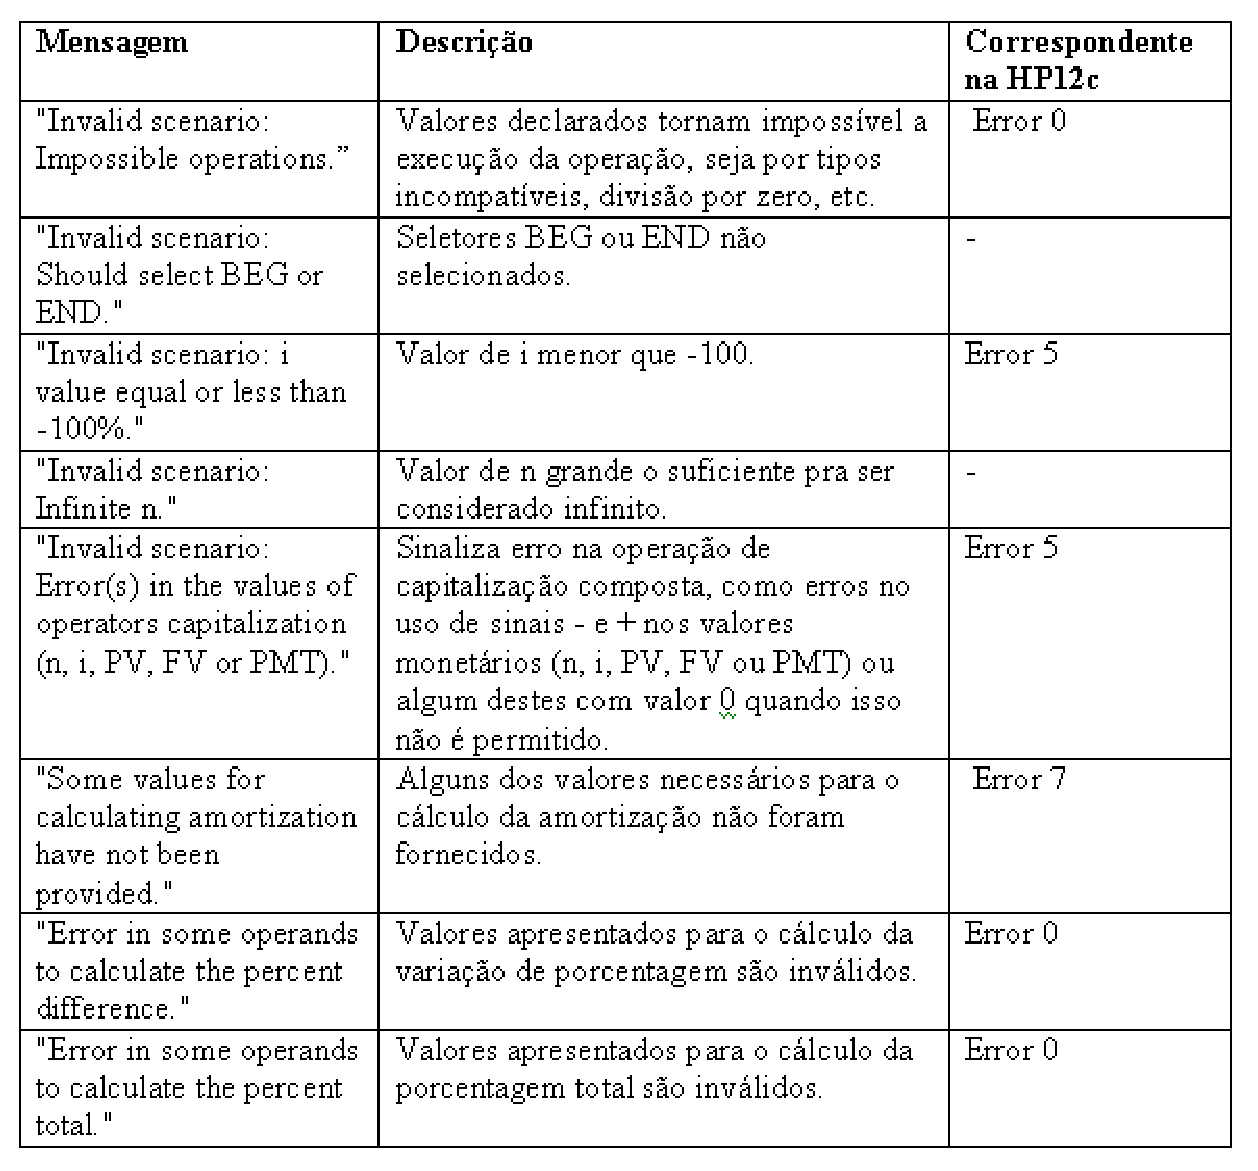
\includegraphics[scale = .7]{tabErro1.eps}
%  \includegraphics[scale=0.5]{bigchart.eps}
\caption{\it Mapeamento de Erros da Biblioteca}
\label{tabErros1} 
\end{figure}

\begin{figure}[!h]
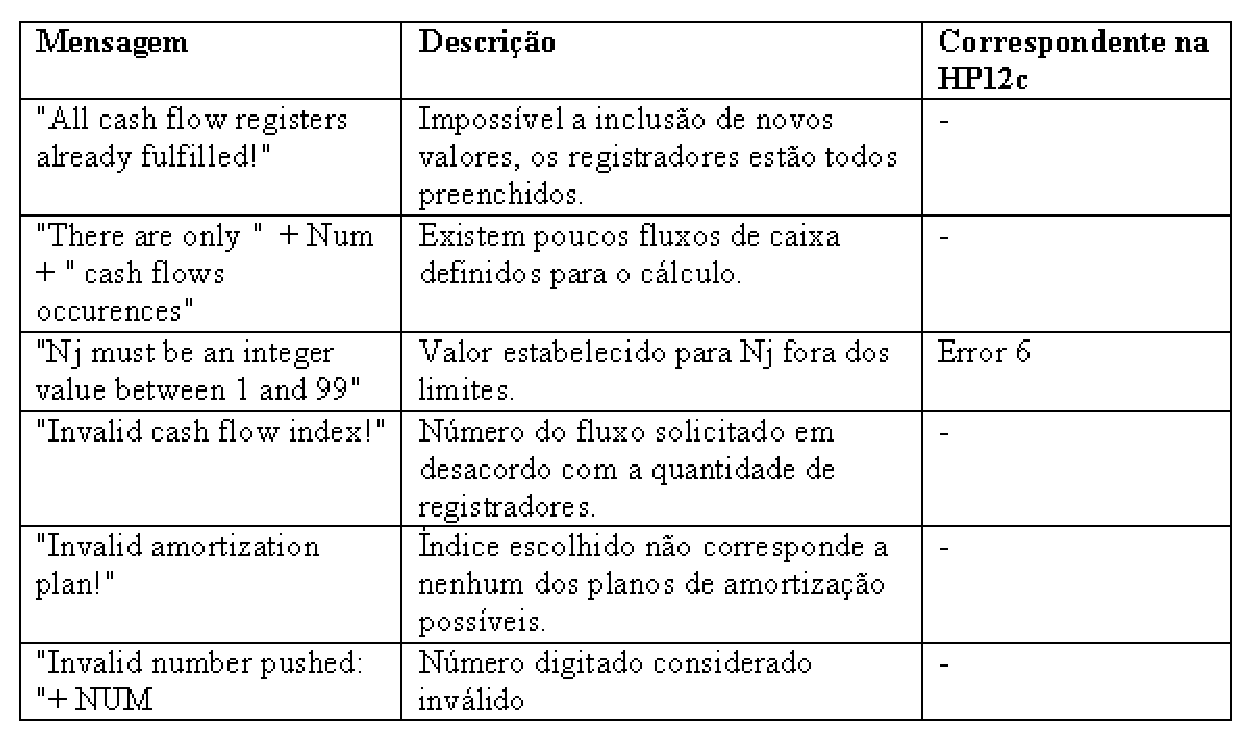
\includegraphics[scale = .7]{tabErro2.eps}
\caption{\it Mapeamento de Erros da Calculadora}
\label{tabErros2}
\end{figure}

\chapter{Diagrama de Classes}

Aqui temos a visualização dos principais componentes da calculadora financeira apresentados em um diagrama de classes. Os principais módulos e pacotes estão apresentados nas Figuras \ref{view} e \ref{model}.

\begin{figure}[!h]
 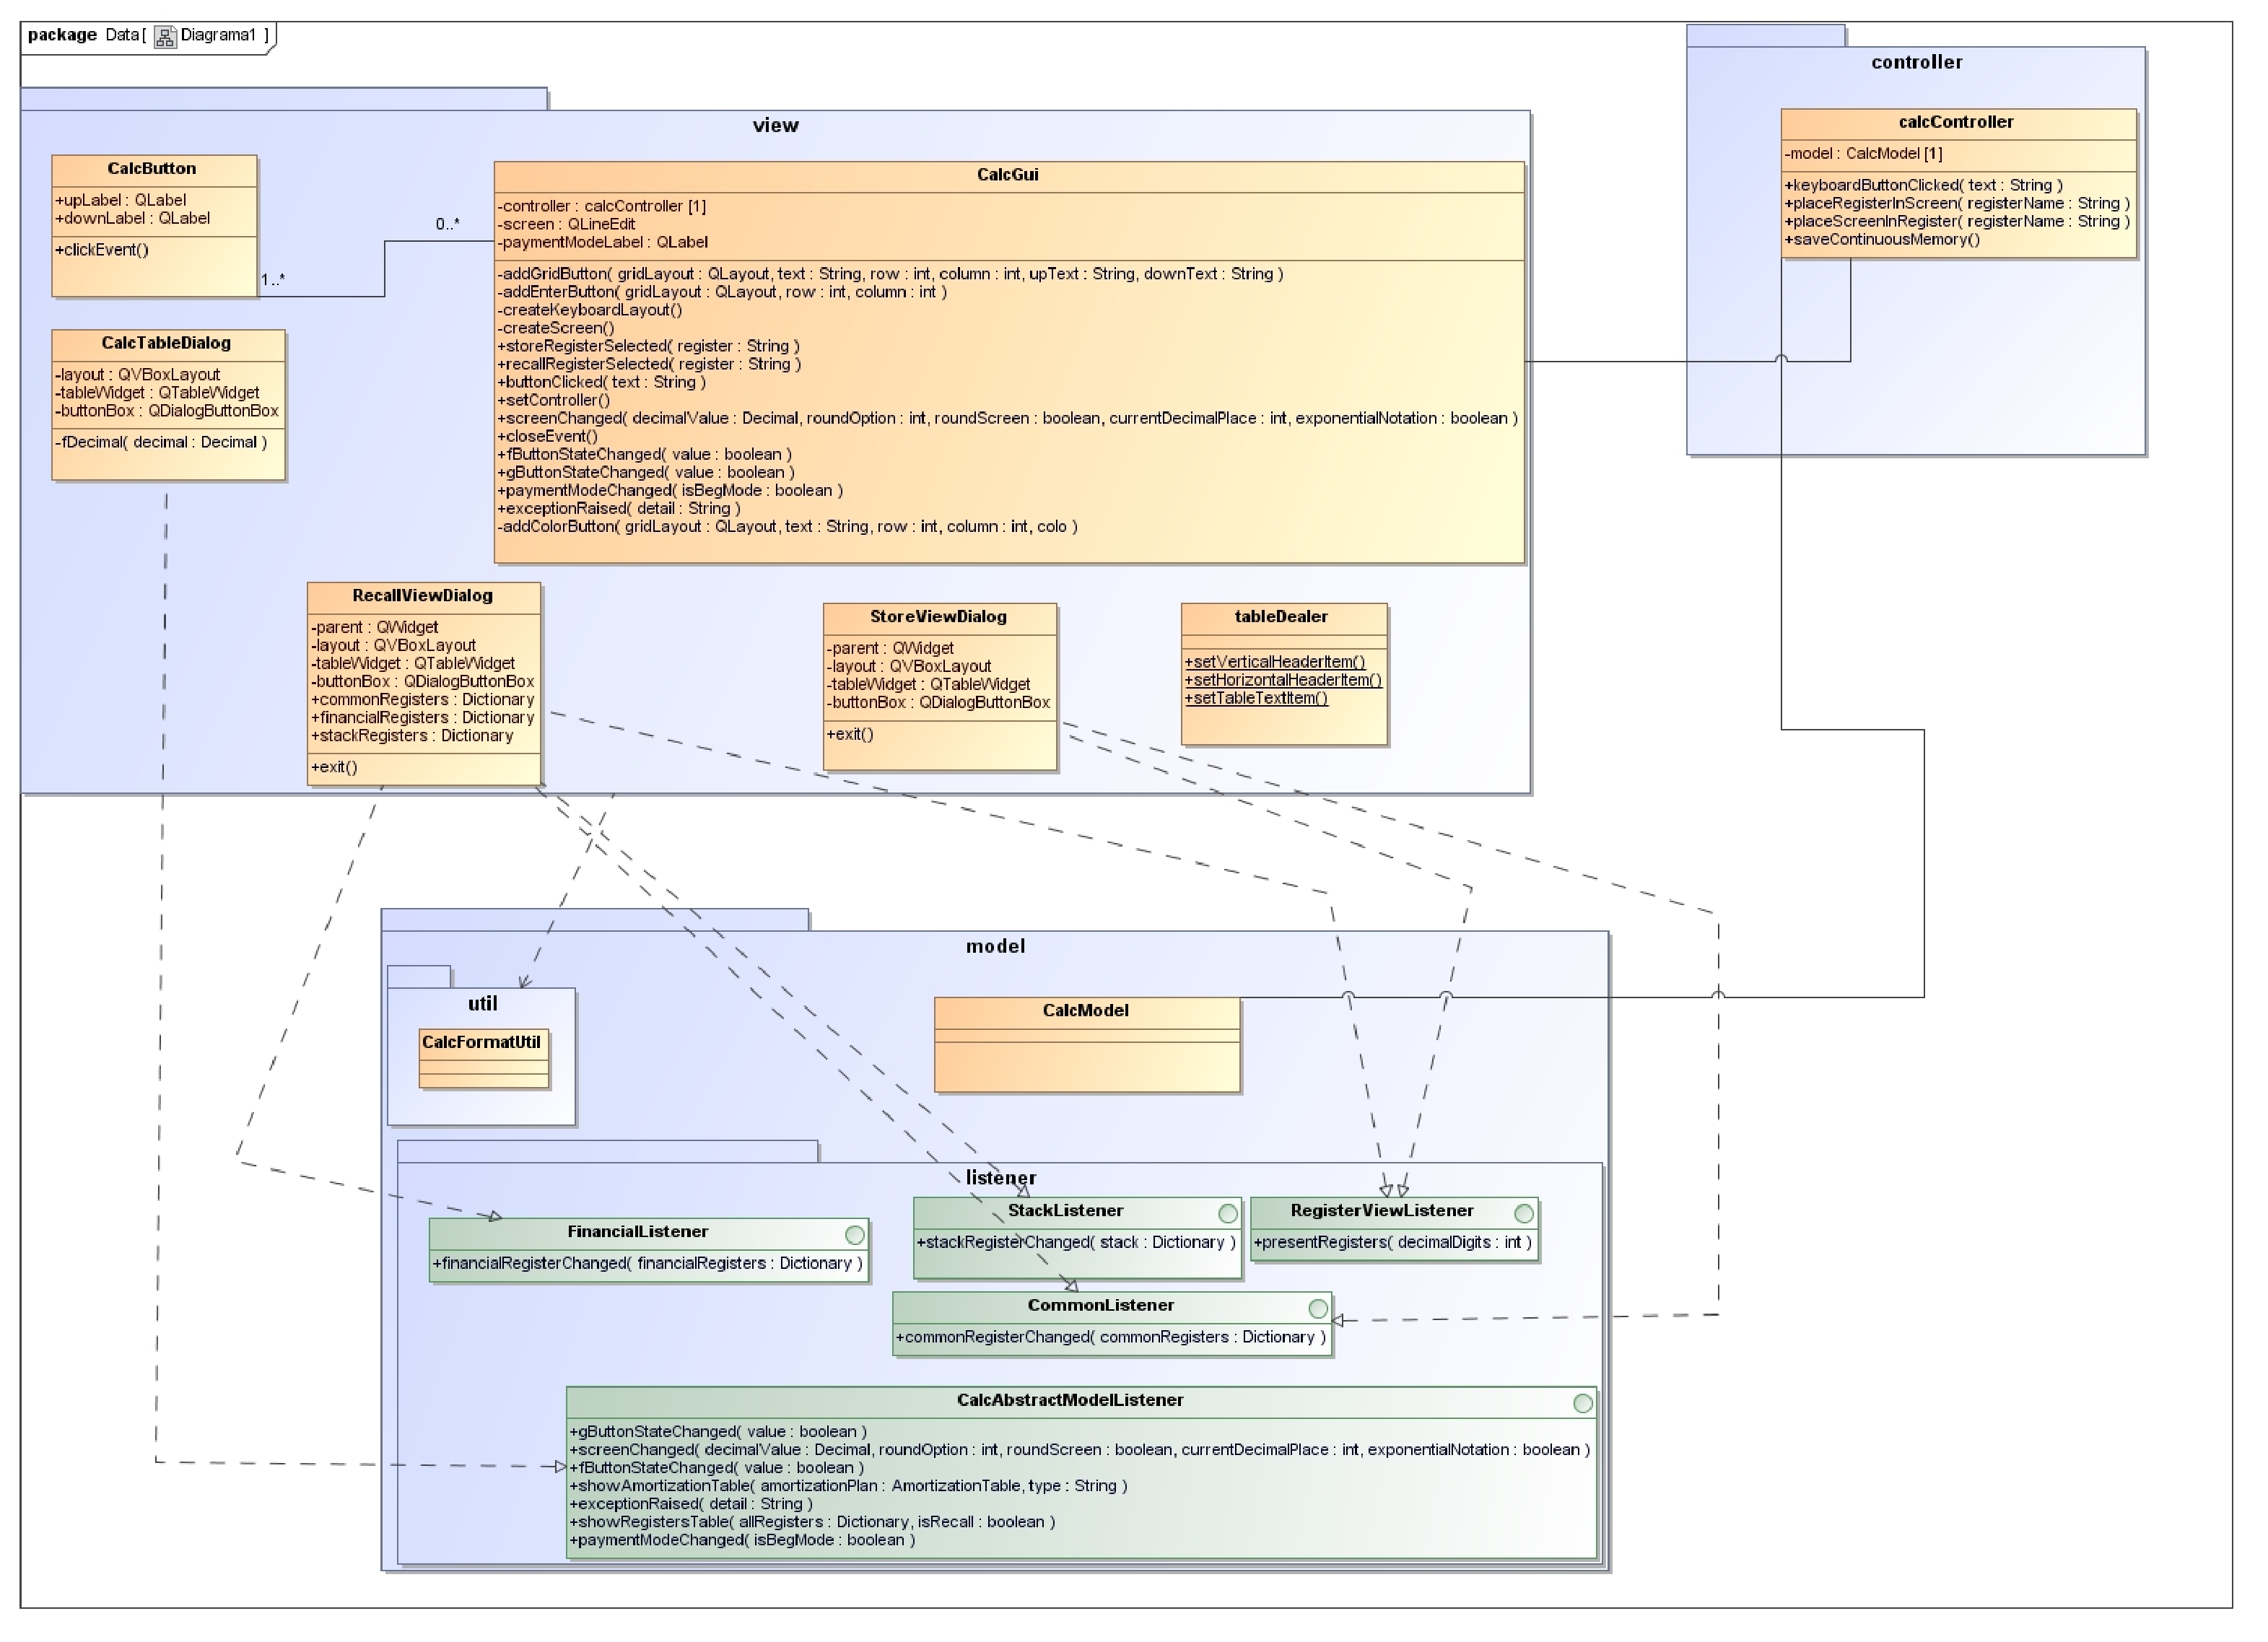
\includegraphics[scale=0.3]{Diagrama1.eps}
 \caption{\it Pacote view e controller e ligações com o pacote model.} \label{view}
\end{figure}

\begin{figure}[!h]
 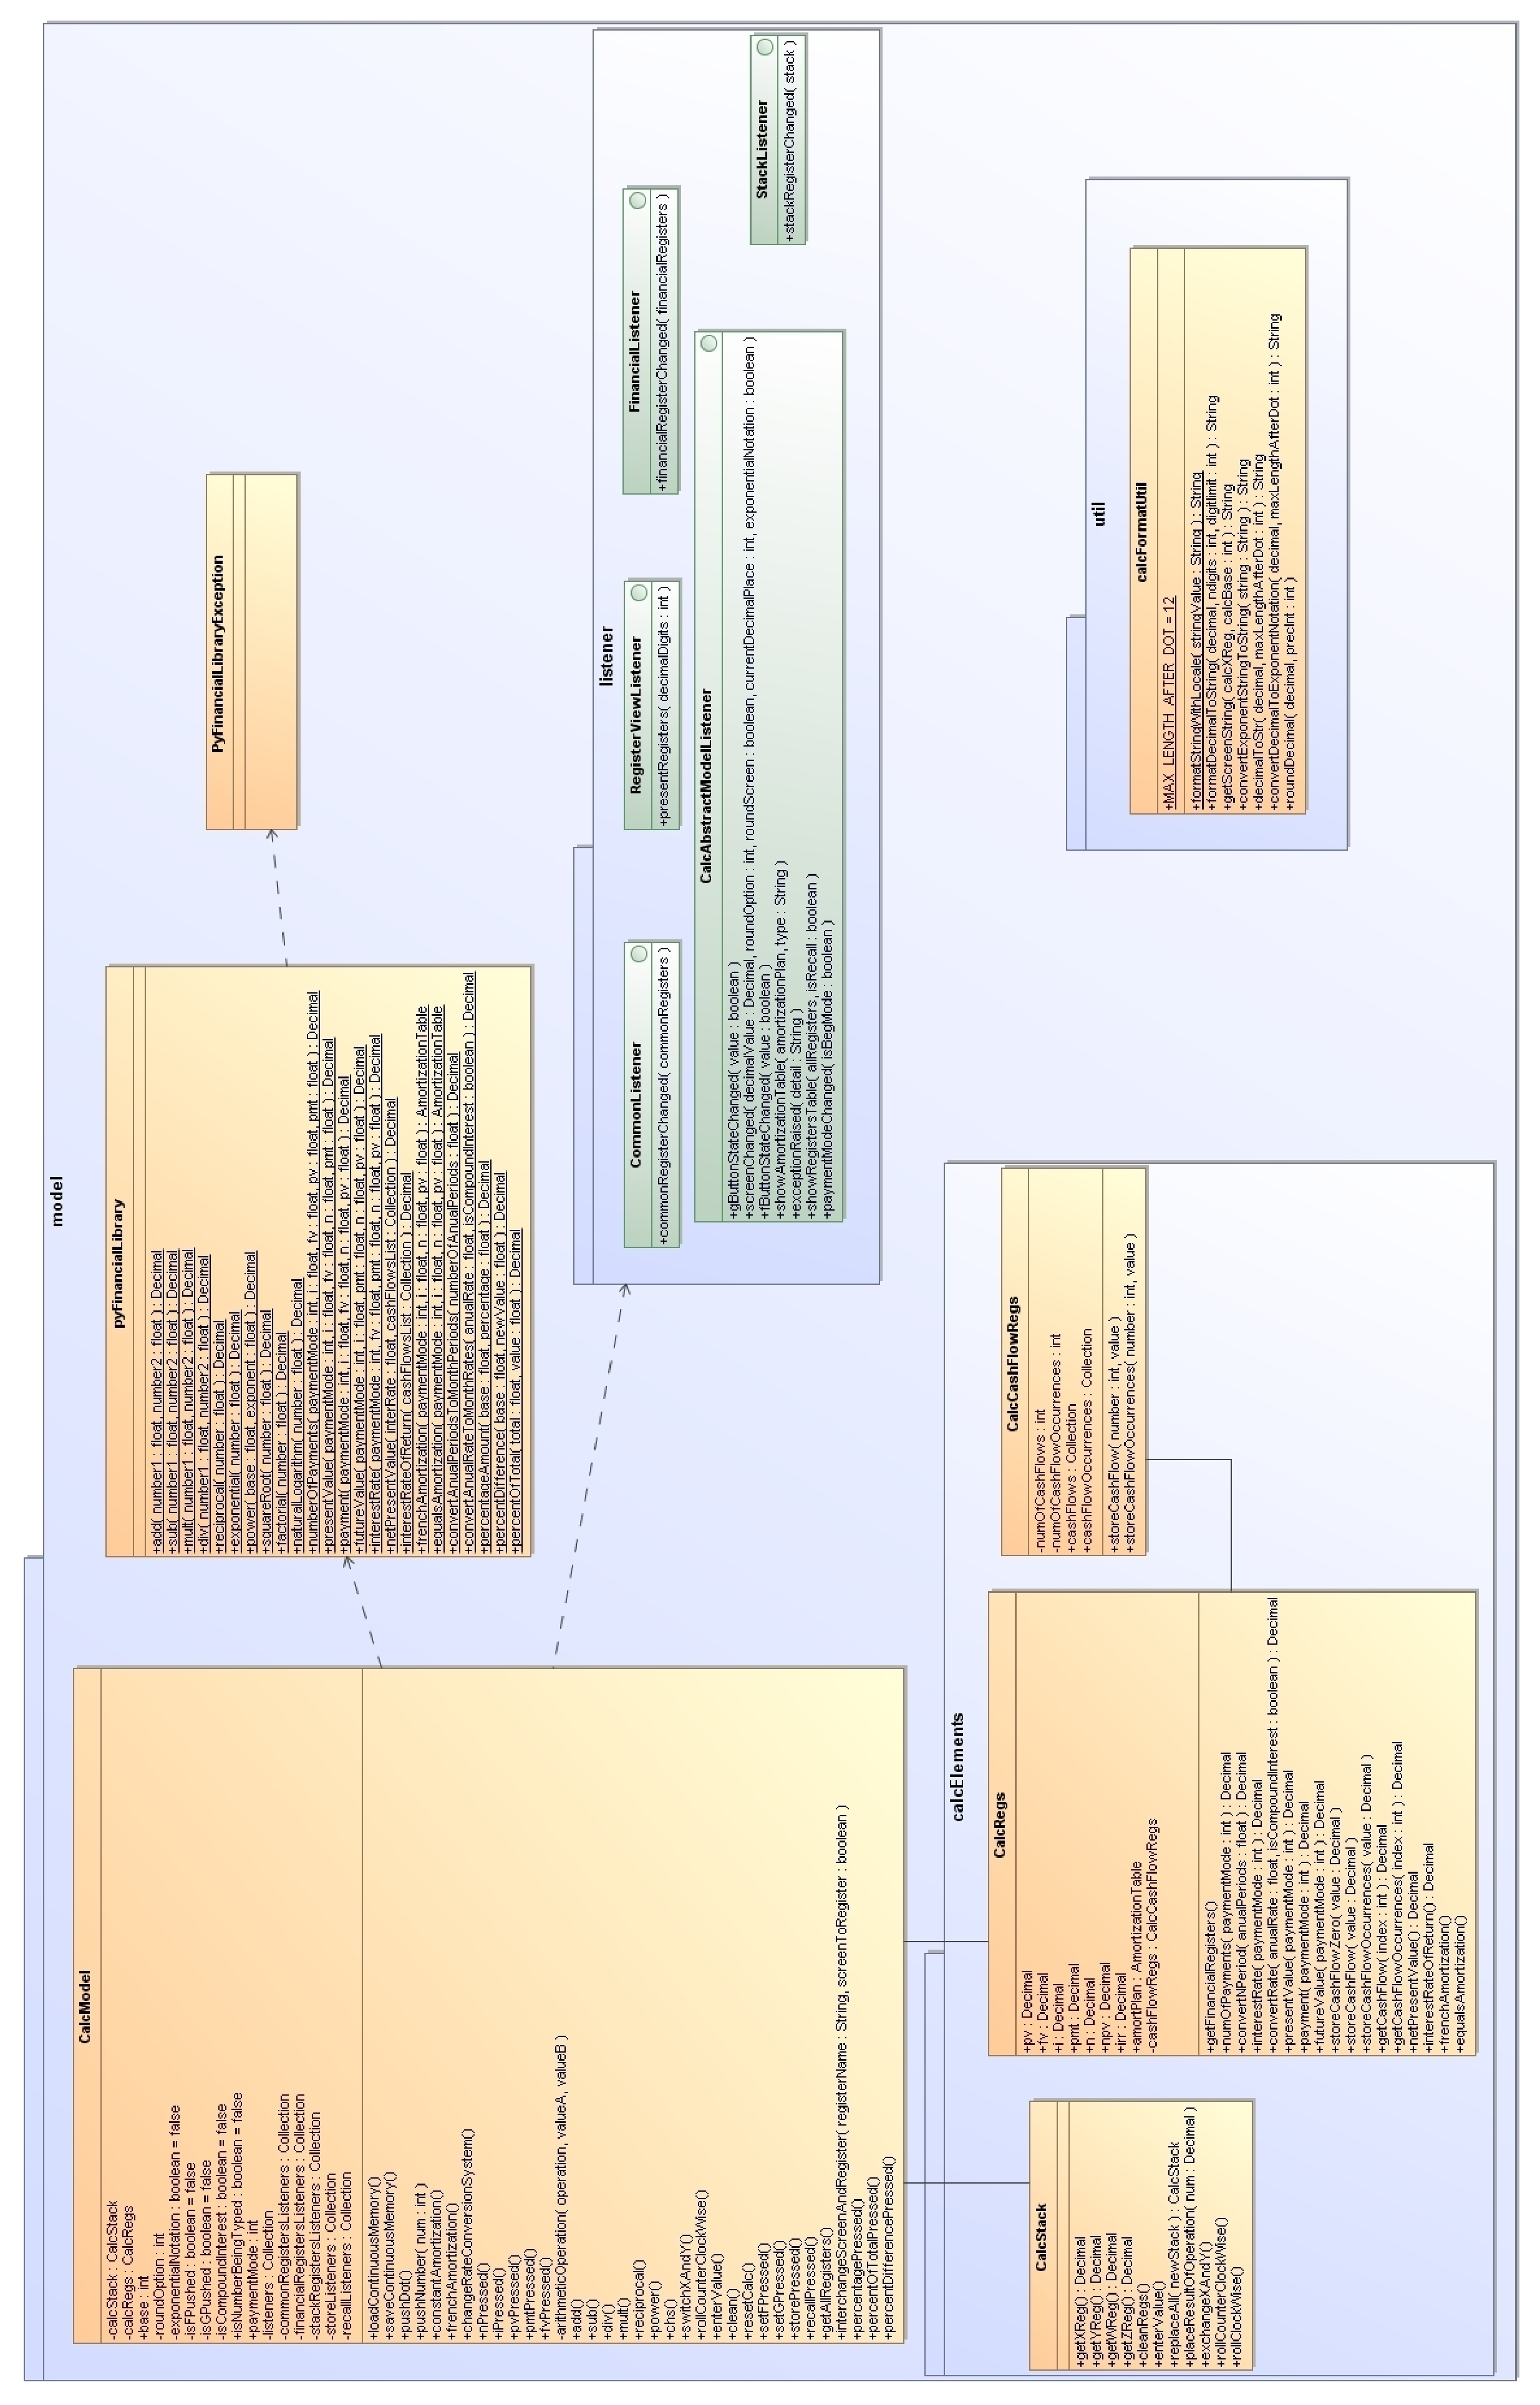
\includegraphics[scale=0.25]{model.eps}
 \caption{\it Pacote model.} \label{model}
\end{figure}









% \chapter{Telas da Aplicação}

\subsection{Tela Principal}

\begin{figure}[!h]
 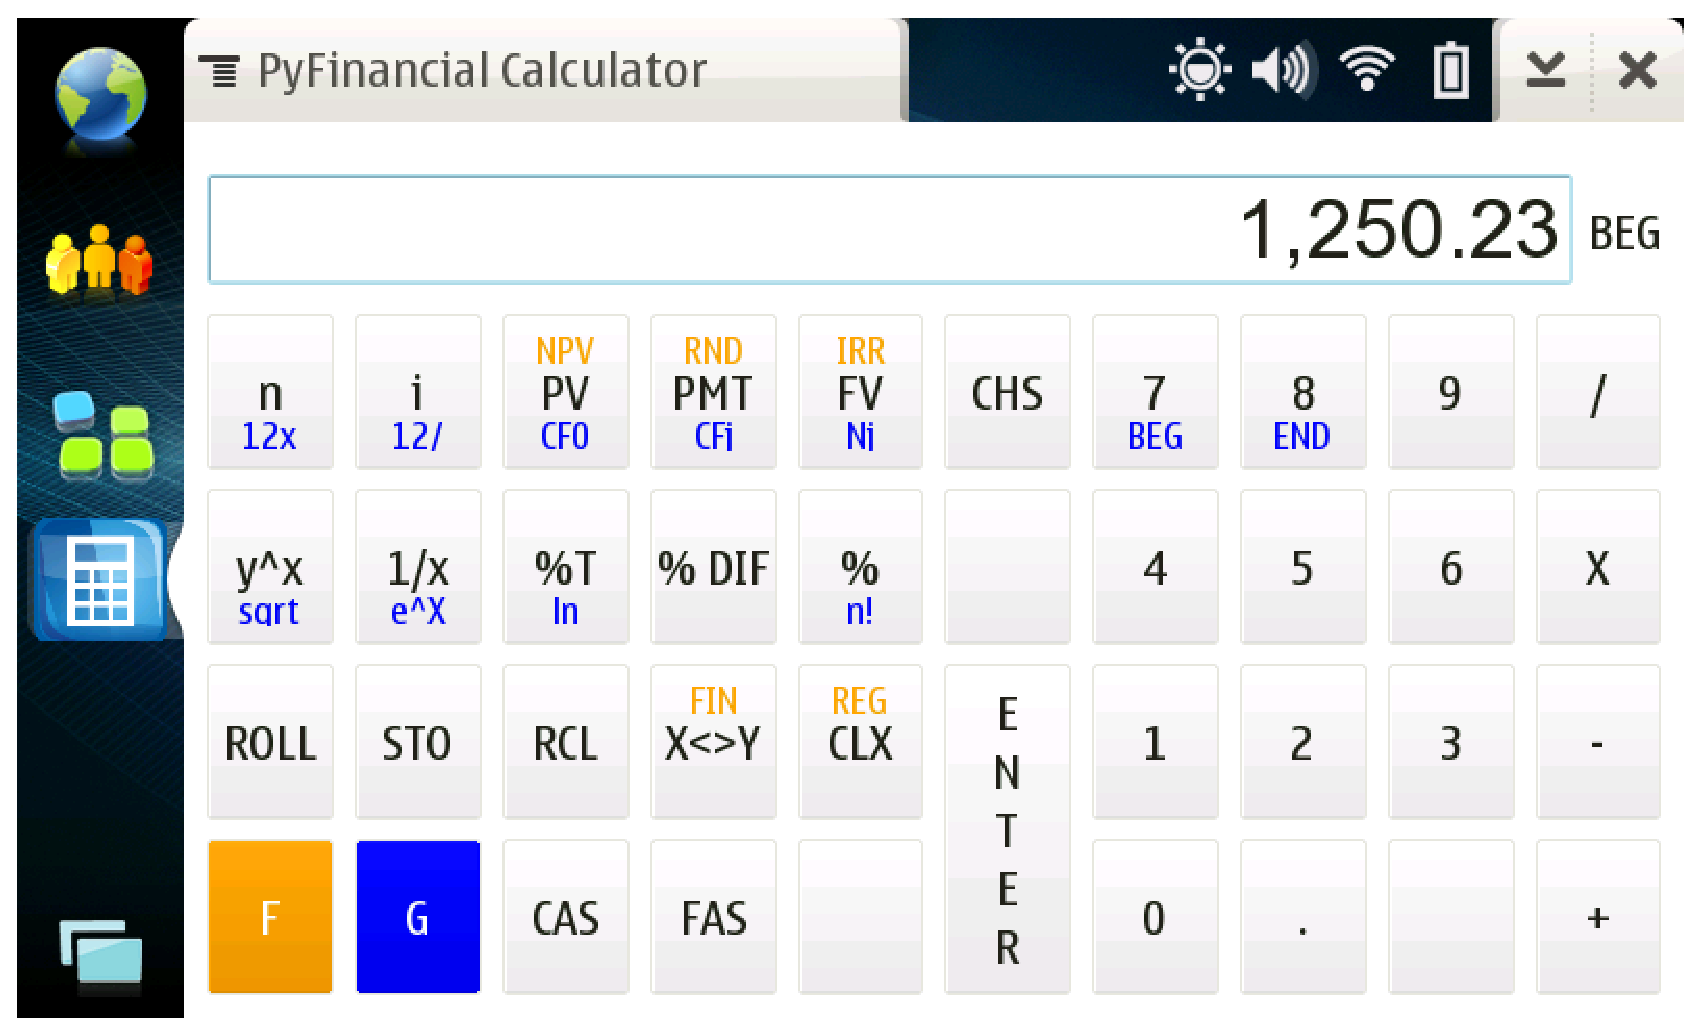
\includegraphics[scale=0.55]{tela_principal.eps}
 \caption{\it Tela principal da calculadora.} \label{tab:tela_principal}
\end{figure}

Tela principal da aplicação que permite o usuário ter acesso a todas as funcionalidade
implementadas pela calculadora. É atraves do mostrador da calculadora que o usuário irá
receber o resultado da maioria das funcões.


\subsection{Tela de Exceção}

\begin{figure}[!h]
 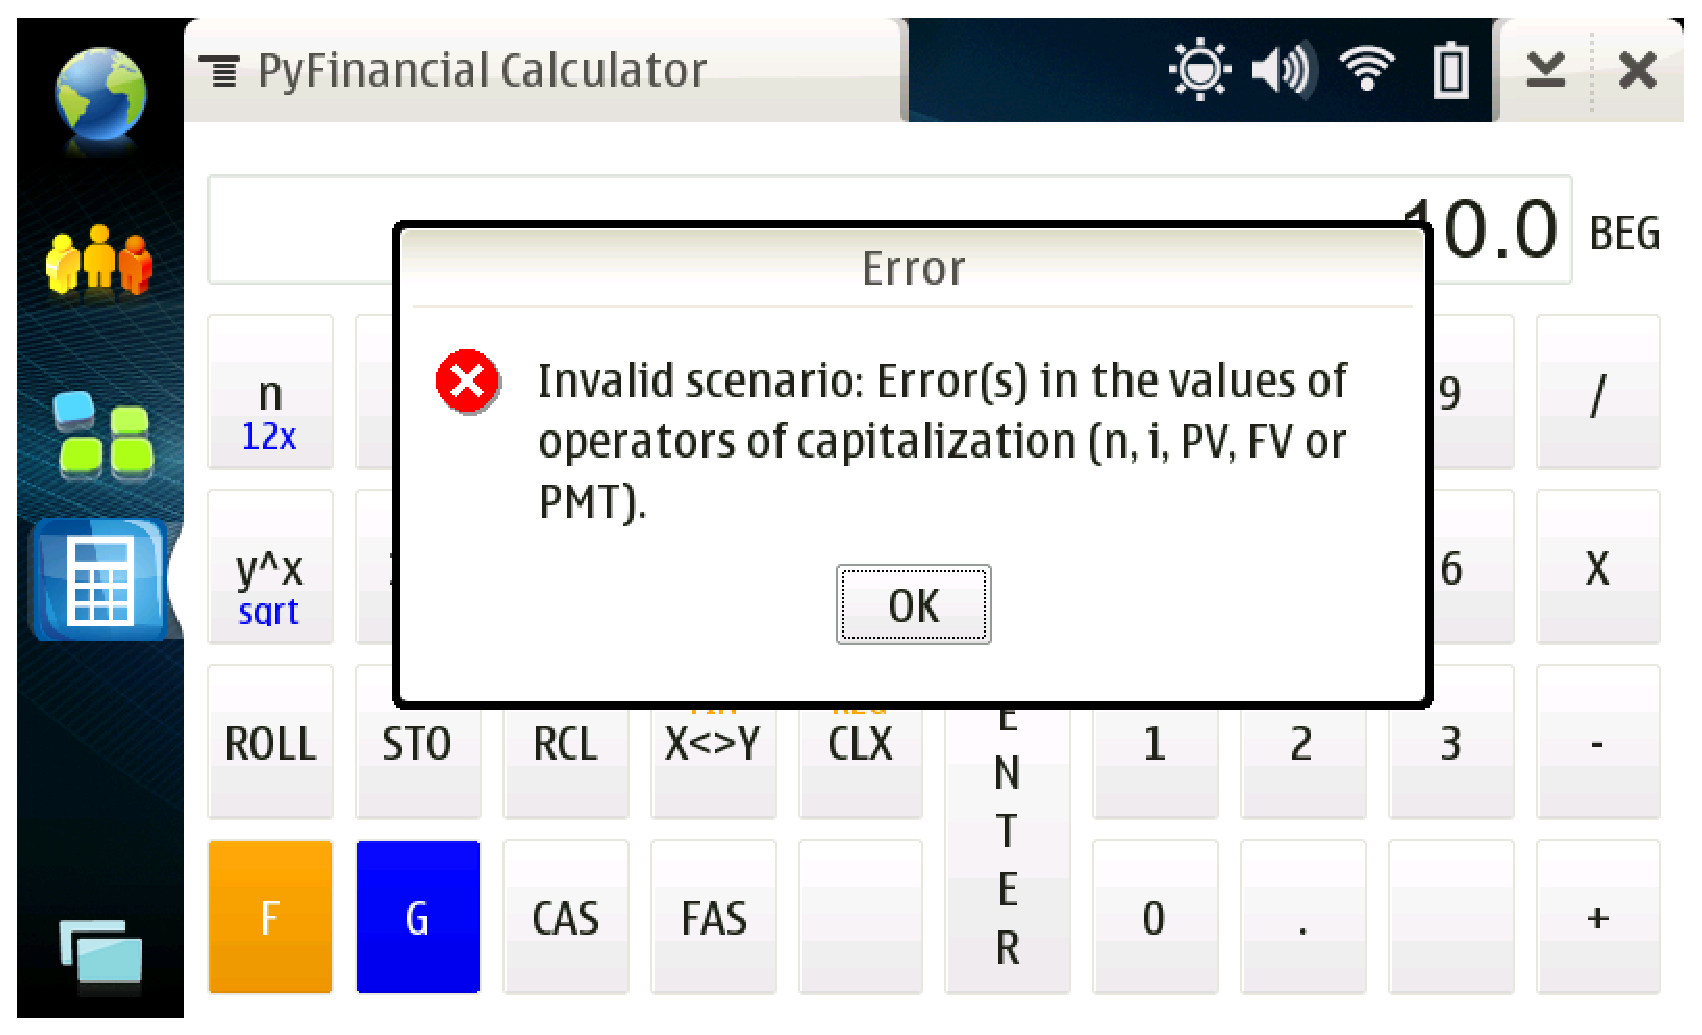
\includegraphics[scale=0.55]{tela_error.eps}
 \caption{\it Tela de exceção.} \label{tab:tela_error}
\end{figure}

Tela principal após uma exceção ser gerada. Um \textit{box} é aberto para mostrar ao usuário a
mensagem de erro.


\subsection{Telas de Amortização}

\begin{figure}[!h]
 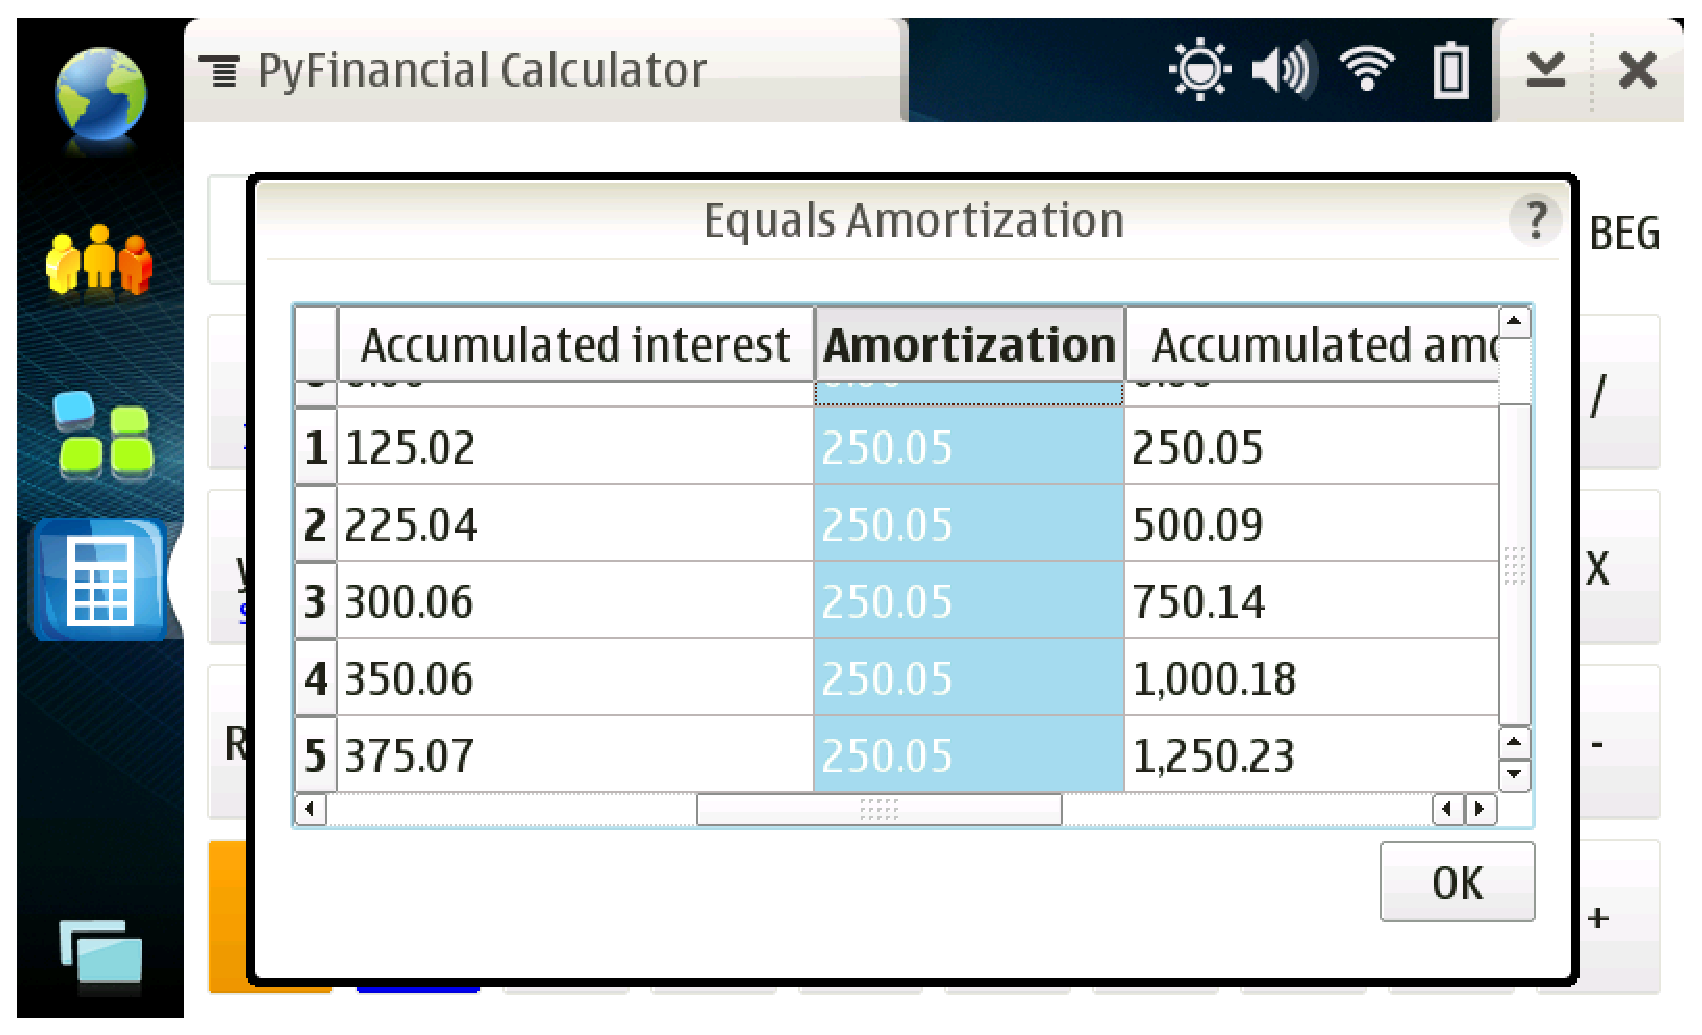
\includegraphics[scale=0.55]{tela_cas.eps}
 \caption{\it Tela de amortização constante.} \label{tab:tela_cas}
\end{figure}

\begin{figure}[!h]
 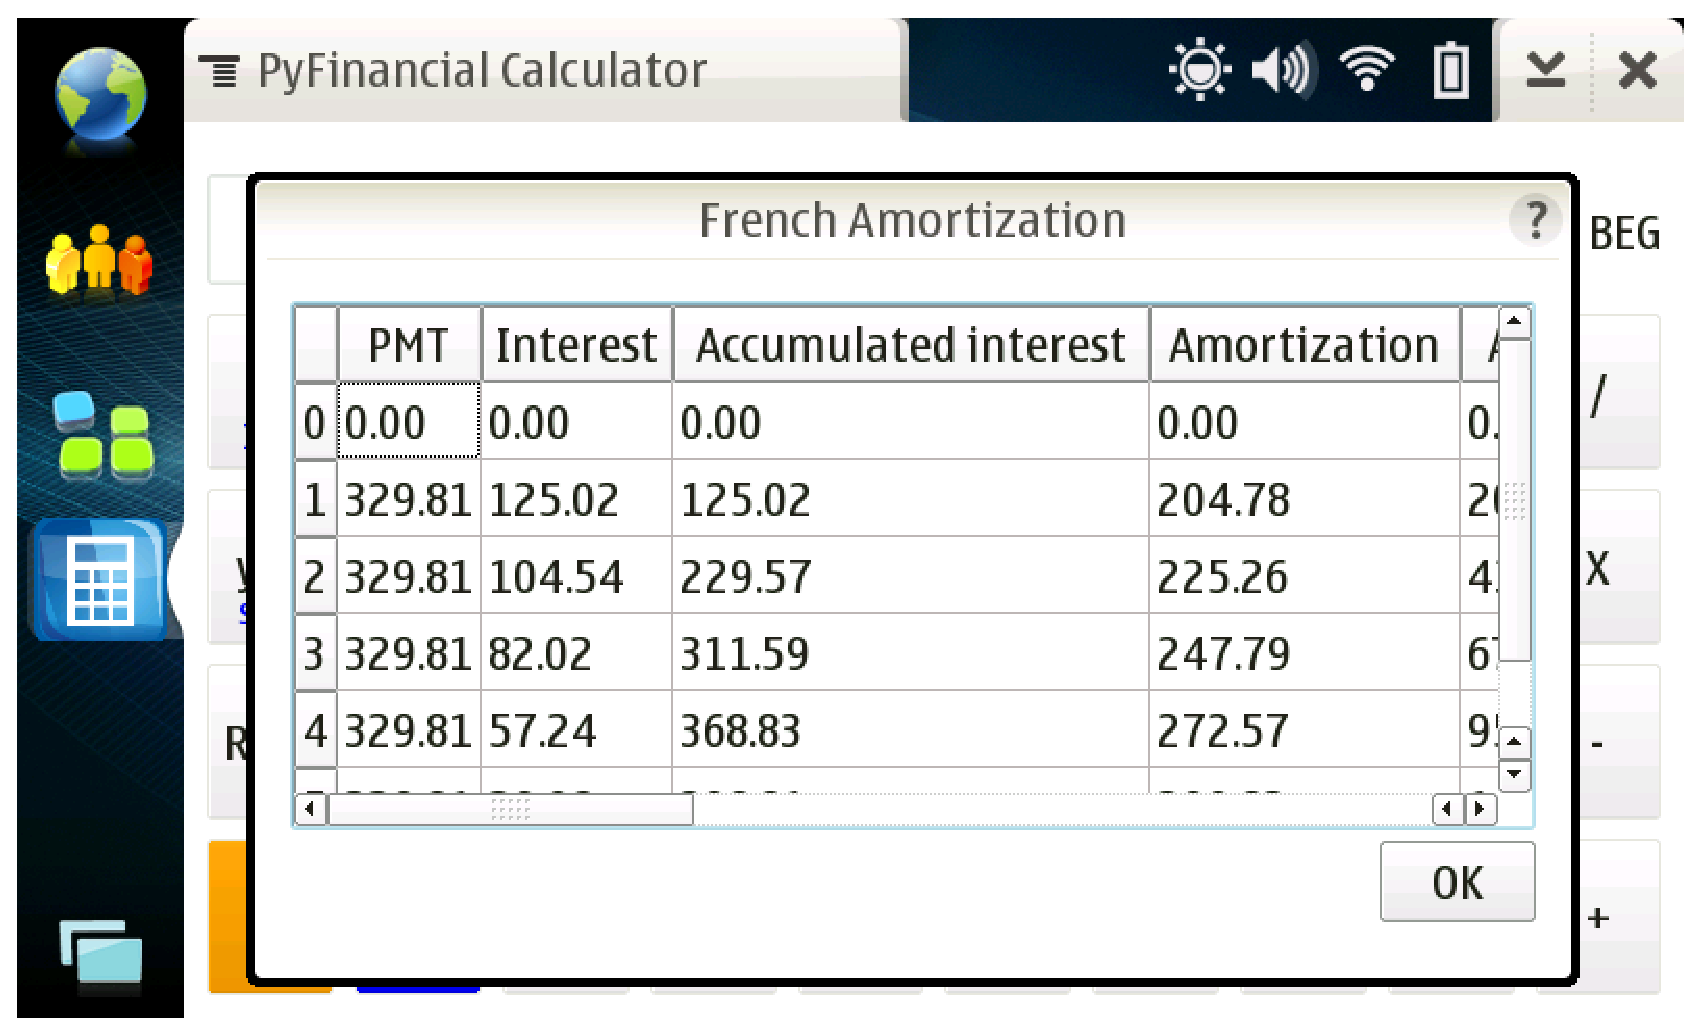
\includegraphics[scale=0.55]{tela_fas.eps}
 \caption{\it Tela de amortização francesa.} \label{tab:tela_fas}
\end{figure}


As telas de amortização apresentam no formato de tabela o resultado de uma calculo de
amortização constate ou francesa.


\subsection{Telas de Recall}

\begin{figure}[!h]
 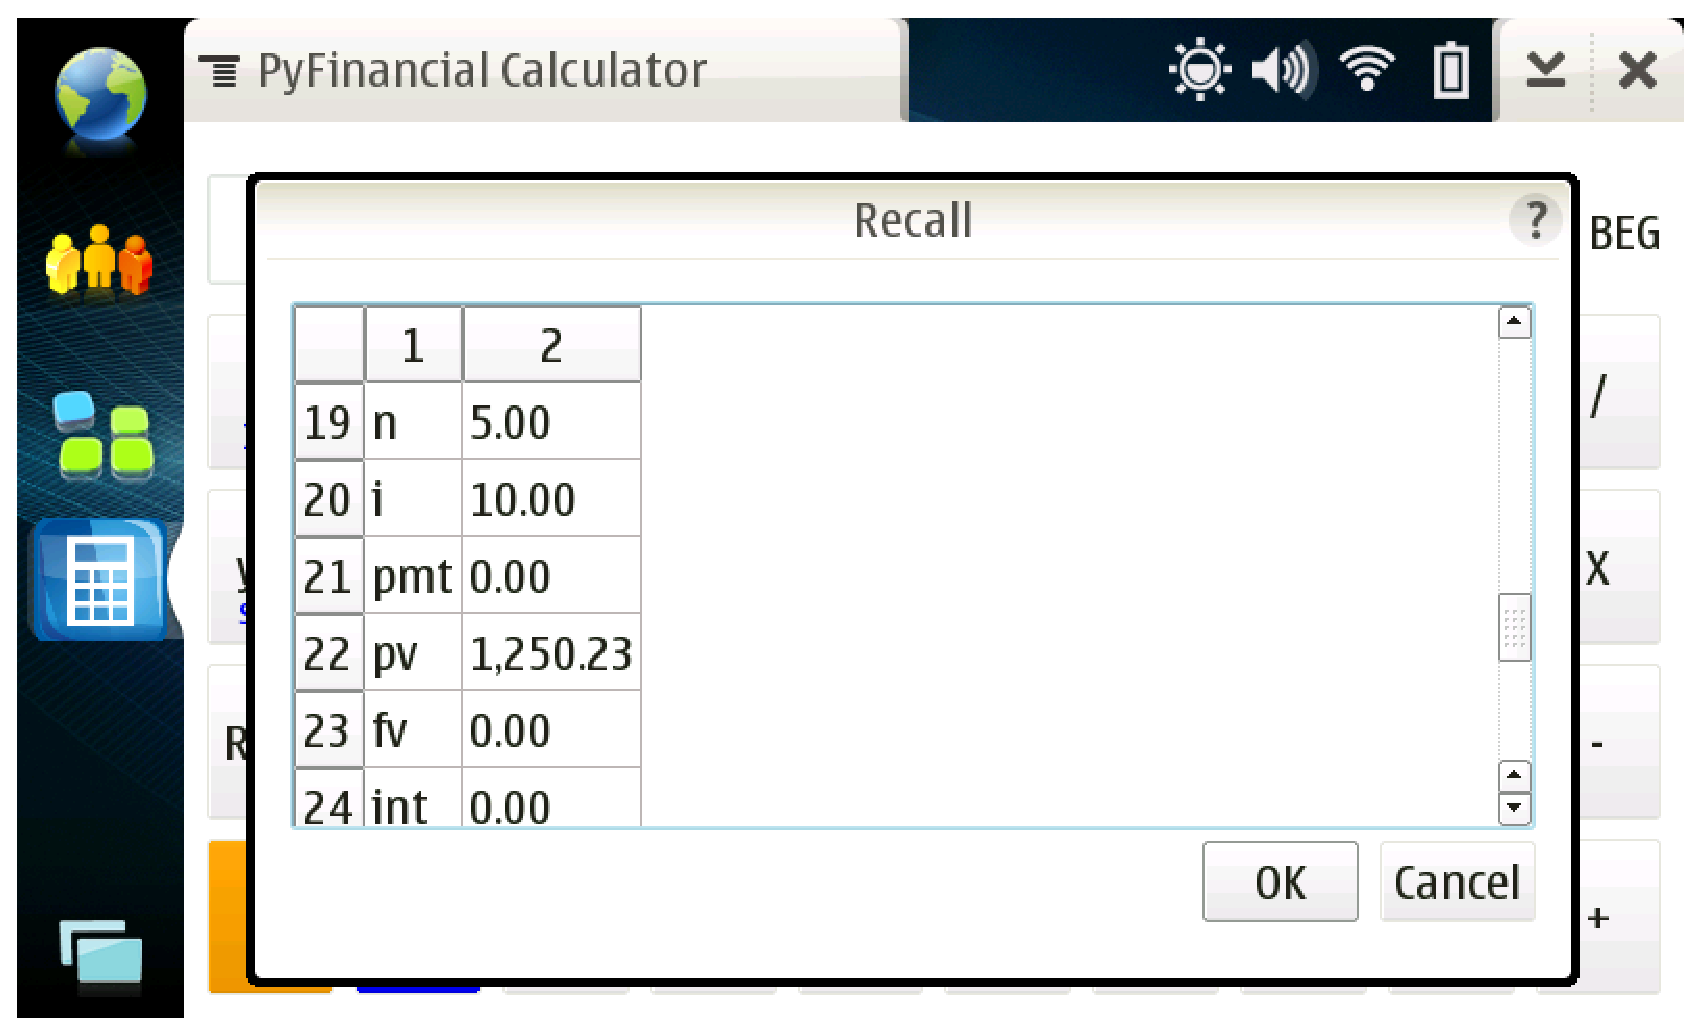
\includegraphics[scale=0.55]{tela_recall.eps}
 \caption{\it Tela de \textit{recall} de registradores.} \label{tab:tela_recall}
\end{figure}

A tela de \textit{Recall} serve para o usuário selecionar um registrador da calculadora e o valor
dele será mandado para o mostrador quando o ele clicar em \textit{OK}. Dessa forma, a pessoa poderá
utilizar o valor de um registrador em novos cálculos.

Existe também uma tela de \textit{Store}, com o mesmo design da tela de \textit{Recall}, que permite que o
usuário faça o inverso, ou seja, armazene o valor do mostrador em um registrador.


% ------------------  Bibliografia  ------------------- %
%% Bibliografia

\bibliographystyle{sbc} % estilo de bibliografia
\bibliography{referencias.bib} % arquivos com as entradas bib.





\end{document}
